\section{Definition of Antiderivatives and the Mean Value Theorem}
In previous chapters, we have learned the derivatives of several common functions, and how to use a set of differentiation rules to find the derivatives of functions that are built from common functions.  We are now like wizards that are ever powerful.  Given any function, no matter how complicated they are, we can repeatedly use the set of rules to produce its derivative.  Now we turn our focus to finding \textit{antiderivatives}, which is the \textit{reverse} of finding derivatives.  Given an arbitrary function, we would like to know \textit{which function has it as the derivative}.  The process of finding antiderivatives is called \textit{antidifferentiation}.  For example, suppose we are given a function
\[f(x) = 4x^3\]
since we know that $\frac{d}{dx}x^4 = 4x^3 = f(x)$, we say that $F(x) = x^3$ is an \textit{antiderivative} for $f(x)$.  However, notice that $\frac{d}{dx}(x^4+1) = 4x^3 = f(x)$, so $G(x) = x^4+1$ is also an antiderivative for $f(x)$.  Now it seems that we are doomed: there are multiple functions that has the same derivative $4x^3$, so how can we be sure that we can find or have found all of them?  Fortunately, we have a very important theorem that can guide us through this mess.

\begin{theo}[Mean Value Theorem]{thm: MVT}
    Let $f(x)$ be a function that is continuous in $[a, b]$ and differentiable in $(a, b)$, then there exists $c$ in $(a, b)$ such that
    \[f'(c) = \frac{f(b)-f(a)}{b-a}\]
\end{theo}
This theorem can be better explained by the graph in the next page.  There are two points $A(a, f(a))$ and $B(b, f(b))$ on the curve of a differentiable function $f(x)$.  Then $\frac{f(b)-f(a)}{b-a}$ is the slope of the secant line shown in red.  What Mean Value Theorem tells us is that you can always find a point $C(c, f(c))$ on the curve between $A$ and $B$, such that the tangent line over $C$ has the same slope as the secant line, such as the blue line in the graph.  Though this theorem seems very intuitive, it can help us prove an essential lemma.

\begin{figure}[ht]
    \centering
    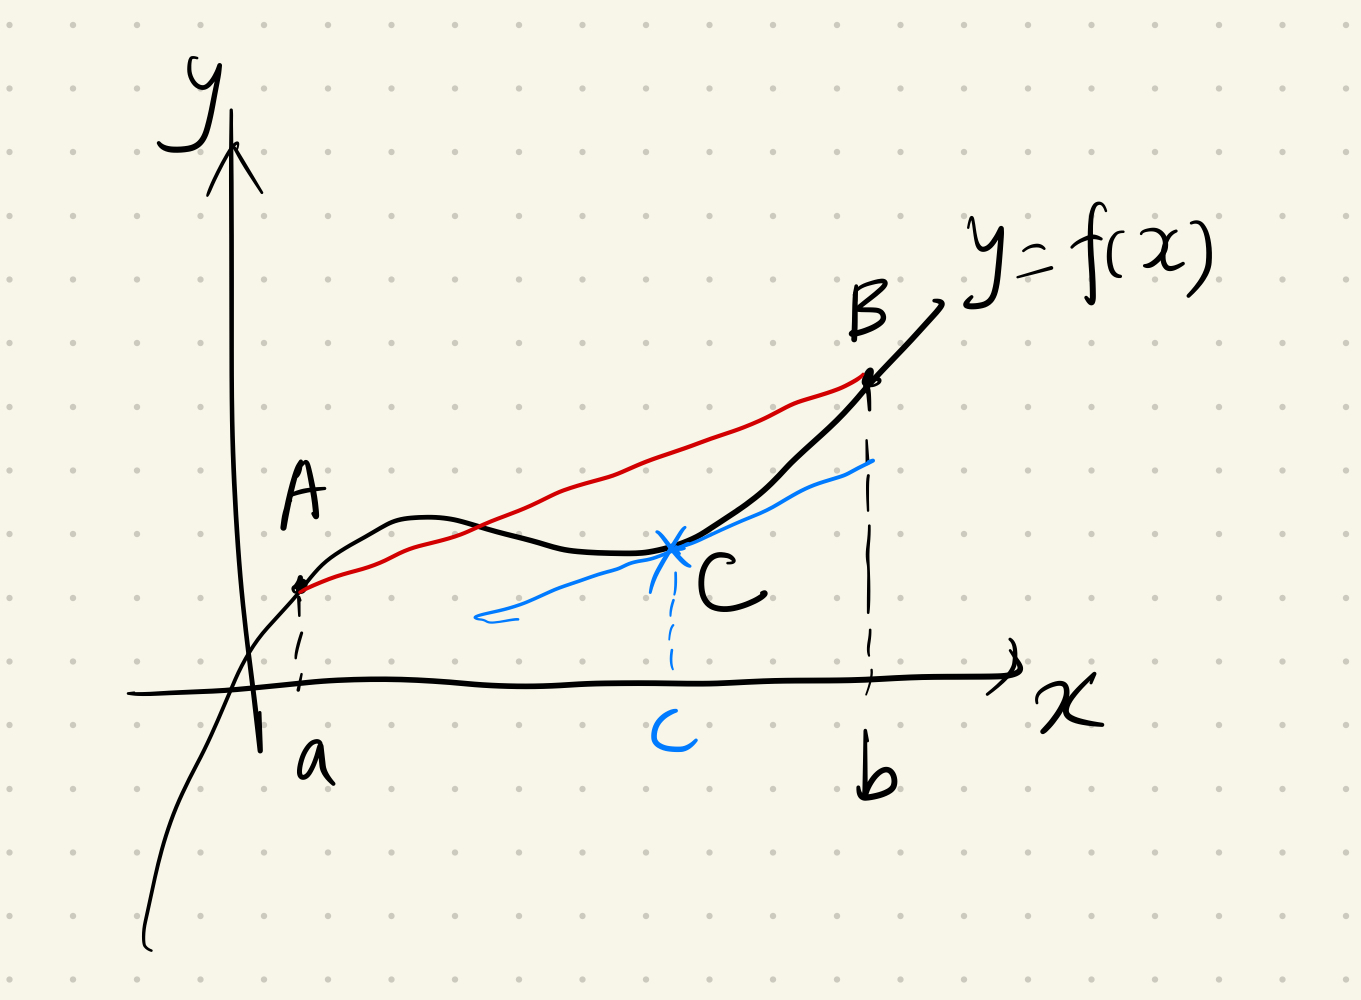
\includegraphics[width = 0.5\textwidth]{figures/chap 06/MVT.png}
\end{figure}

\newpage

\begin{lem}[The Antiderivative of Zero]{lem: zero_integral}
    If $f'(x) = 0$ within $(a,b)$, then $f(x) = C$ within $(a,b)$, where $C$ is a constant.
\end{lem}

\begin{prf}[]{pf: zero_integral}
    We use proof by contradiction.  
    
    Suppose $f'(x) = 0$ within $(a, b)$ but $f(x)$ is \textit{not} constant within $(a, b)$.  Then we can find two extra points $(c, f(c))$ and $(d, f(d))$ where $a < c < d < b$ and $f(c) \ne f(d)$.  
    
    Now we know that $f(x)$ is continuous within $[c, d]$ and differentiable within $(c, d)$ (because it is differentiable in $(a, b)$).  So by the Mean Value Theorem, there exists $t$ in $(c, d)$ such that $f'(t) = \frac{f(d)-f(c)}{d-c} \ne 0$, which contradicts the assumption that $f'(x) = 0$ within $(a, b)$.  Therefore, $f(x)$ must be a constant within $(a, b)$. 
\end{prf}

Now we can show the following theorem:

\begin{theo}[Constant of Integration]{thm: C_in_int}
    Suppose $F(x)$ and $G(x)$ are both antiderivatives for $f(x)$, then there exists a constant $C$ so that $G(x) = F(x) + C$.
\end{theo}

\begin{prf}[]{pf: C_in_int}
    We define $H(x) = G(x) - F(x)$.  Then we have $H'(x) = G'(x) - F'(x) = f(x) - f(x) = 0$.  From Lemma \ref{lem: zero_integral}, we thus know that $H(x) = C$ where $C$ is a constant.  Therefore $G(x) = F(x) + C$.
\end{prf}

Therefore, if $F(x)$ is \textit{one} of the antiderivatives for a function $f(x)$, then \textit{all} the antiderivatives for $f(x)$ would be shaped as $F(x) + C$, where $C$ is a unknown constant.  In other words, we only need to strive to find one antiderivative, then add $+C$ in the end and call it a day, without fearing that some other weird function would also be an antiderivative.  In the previous example, the antiderivative of $f(x) = 4x^3$ can then be written as $x^4 + C$.

In previous sections, we used $f'(x)$ or $\frac{d}{dx}f(x)$ to denote the derivative of $f(x)$.  For antiderivatives, we also have a notation written as
\[\int f(x) dx\]
where $\int$ is the integration sign, derived from a elongated "S" standing for summation.  We will talk about the link between antiderivatives and integrals in the next chapter, so up until now please bear with the name.  The function to be antidifferentiated, $f(x)$, is also called the \textit{integrand}.  $dx$ is a symbol that tells us that with respect to what variable are we antidifferentiating.  Later we will introduce its formal name: the \textit{differential}.  Using this new notation, we can now write
\[\int 4x^3 dx = x^4 + C\]
With these new concepts and notations at hand, let us look at some examples of antiderivatives:
\begin{eg}[]{eg: antiderivative}
    Find the following antiderivatives:
    \begin{tasks}(4)
        \task $\int 3 dx$
        \task $\int 2x dx$
        \task $\int 6x^5 dx$
        \task $\int -\frac{1}{x^2} dx$
        \task $\int \cos x dx$
        \task $\int -\sin x dx$
        \task $\int e^x dx$
        \task $\int \frac{1}{x} dx$
    \end{tasks}
\end{eg}

\begin{egsol}[]{egsol: antiderivative}
    \begin{enumerate}[a)]
        \item We know for any constant $k$
        \[\frac{d}{dx}kx = k\]
        so $3x$ is \textit{one} of the antiderivatives of $3$, and we have $\int 3 dx = 3x + C$.
        \item In the power rule for differentiation, we have 
        \[\frac{d}{dx} x^r = r x^{r-1}\]
        where the power decreases by $1$ after differentiation.  This prompts us to guess that the antiderivative for a multiple of $x^r$ should be a multiple of $x^{r+1}$, where the power increases by $1$ after antidifferentiation.  Here we can try guessing $x^2$ and verify that
        \[\frac{d}{dx} x^2 = 2x\]
        which gets to our desired function.  Therefore, $x^2$ is \textit{one} of the antiderivatives for $2x$ and we have $\int 2x dx = x^2 + C$.
        \item Similar to the previous subproblem, since $6x^5$ is a multiple of $x^5$, we can use the reverse of power rule and try guessing something like $x^6$ and verify that
        \[\frac{d}{dx} x^6 = 6x^5\]
        so we know $x^6$ is \textit{one} of the antiderivatives for $6x^5$, and we have $\int 6x^5 dx = x^6 + C$.
        \item Here $-\frac{1}{x^2}$ can actually be rewritten as $-x^{-2}$, so it is a multiple of power of $x$.  Therefore, we can try guessing $x^{-1}$ for its antiderivative and verify that
        \[\frac{d}{dx}x^{-1} = -x^{-2}\]
        so that $x^{-1}$ indeed an antiderivative for $-x^{-2}$.  Therefore we have $\int -\frac{1}{x^2} dx = -\frac{1}{x} + C$.
        \item We have known by heart that
        \[\frac{d}{dx}\sin x = \cos x\]
        so we already know $\sin x$ is \textit{one} of the antiderivatives for $\cos x$.  Therefore we have $\int \cos x dx = \sin x + C$.
        \item Likewise, we already know that 
        \[\frac{d}{dx}\cos x = -\sin x\]
        so $\cos x$ is \textit{one} of the antiderivatives for $-\sin x$, and we have $\int -\sin x dx = \cos x + C$.
        \item $e^x$ is a special function where 
        \[\frac{d}{dx} e^x = e^x\]
        therefore $e^x$ is an antiderivative for $e^x$ itself, so we have $\int e^x dx = e^x + C$.
        \item Recall than the derivative of $\ln x$
        \[\frac{d}{dx} \ln x = \frac{1}{x}\]
        therefore intuitively, we would say that $\ln x$ is an antiderivative for $\frac{1}{x}$.  However, this is just part of the answer.  Notice that when we differentiate $\ln x$ and get $1/x$, we are implicitly assuming that $x$ can only take up positive values in both functions, since $\ln x$ is defined only for $x > 0$.  However, when we are antidifferentiating $1/x$, since $1/x$ is defined for all non-zero real numbers, we would also want the resulting antiderivative to be defined for all non-zero real numbers.  This can be done by looking into the function $\ln |x|$.  Note that when $x > 0$:
        \[\frac{d}{dx} \ln |x| = \frac{d}{dx} \ln x = \frac{1}{x}\]
        and when $x < 0$:
        \[\frac{d}{dx} \ln |x| = \frac{d}{dx} \ln (-x) = \frac{1}{-x}(-1) = \frac{1}{x}\]
        therefore, $\ln |x|$ is indeed an antiderivative for $1/x$, and it is also defined for all non-zero real numbers.  In the end, we would write $\int \frac{1}{x} dx = \ln |x| + C$.
    \end{enumerate}
\end{egsol}

\bigskip

Eminent students may argue that $\ln |x| + C$ does not actually cover all possible antiderivatives for $\frac{1}{x}$, since the following function also has derivative $\frac{1}{x}$:
\[F(x) = \begin{cases} \ln |x| + C_1, x > 0 \\ \ln |x| + C_2, x < 0 \end{cases}\]
Indeed, the "$+C$" trick breaks down here.  This is because when we were proving Theorem 6.3, the argument that $G'(x) - F'(x) = f(x) - f(x) = 0$ is only valid if $f(x)$ exists everywhere, while here $1/x$ is undefined at $x = 0$.  However, in this course we acknowledge that this weakness exists and continue to use $\ln |x| + C$ for simplicity.

\bigskip

\begin{ex}[]{ex: antiderivative}
    Find the following antiderivatives:
    \begin{tasks}(4)
        \task $\int 0~dx$
        \task $\int dx$
        \task $\int 2dt$
        \task $\int \frac{1}{2\sqrt{x}} dx$
        \task $\int \frac{2}{3\sqrt[3]{x}} dx$
        \task $\int \frac{1}{1+x^2} dx$
        \task $\int 2^x \ln 2~dx$
        \task $\int \sec^2 x dx$
    \end{tasks}
\end{ex}

\begin{exsol}[]{exsol: antiderivative}
    \begin{enumerate}[a)]
        \item In Lemma 6.2, we showed that the antiderivative of $0$ is a constant function $C$, so $\int 0~dx = C$.
        \item Here $\int dx$ is the shorthand of $\int 1 dx$.  Based on previous observations, we would guess and verify that $x$ is one antiderivative for $1$.  Therefore we have $\int dx = x + C$.
        \item Notice that here we are antidifferentiating with respect to $t$ instead of $x$, since the differential is $dt$ instead of $dx$.  Based on previous observations, we would guess and verify that $2t$ is one antiderivative for $2$.  Therefore we have $\int 2dt = 2t + C$.
        \item Here $\frac{1}{2\sqrt{x}}$ can be rewritten as $\frac{1}{2}x^{-1/2}$, which is a multiple of $x^{-1/2}$, a power function of $x$.  Therefore, we would naturally guess $x^{-1/2 + 1} = x^{1/2} = \sqrt{x}$ to be one of its antiderivatives, which checks out.  Therefore we have $\int \frac{1}{2\sqrt{x}} dx =  \sqrt{x} + C$
        \item Here $\frac{2}{3\sqrt[3]{x}}$ can be rewritten as $\frac{2}{3}x^{-1/3}$, which is a multiple of $x^{-1/3}$, a power function of $x$.  Therefore, we would naturally guess $x^{-1/3 + 1} = x^{2/3} = \sqrt[3]{x^2}$ to be one of its antiderivatives, which checks out.  Therefore we have $\int \frac{2}{3\sqrt[3]{x}} dx = \sqrt[3]{x^2} + C$.
        \item We specifically derived the derivatives of inverse trigonometic functions in Chapter 4, where we had the identity
        \[\frac{d}{dx}\arctan x = \frac{1}{1+x^2}\]
        Therefore, $\arctan x$ is one of the antiderivatives for $\frac{1}{1+x^2}$, and we have $\int \frac{1}{1+x^2} dx = \arctan x + C$.
        \item In the section where we talked about derivatives of exponential functions, we had the identity
        \[\frac{d}{dx} a^x = a^x \ln a, \quad \forall a > 0\]
        Therefore, $2^x$ is one of the antiderivatives for $2^x \ln 2$, and we have $\int 2^x \ln 2~dx = 2^x + C$.
        \item If you have memorized this one, you would immediately think of the identity
        \[\frac{d}{dx} \tan x = \sec^2 x\]
        Therefore, $\tan x$ is one of the antiderivatives for $\sec^2 x$, and we have $\int \sec^2 xdx = \tan x + C$.
    \end{enumerate}
\end{exsol}

\newpage
Like differentiation, we also have a set of basic antidifferentiation rules that can aid us in finding antiderivatives, which we list below:

\begin{itemize}
    \item Constant rule:
    \[\int k dx = kx + C, \quad \text{where }k\text{ is a constant}\]
    \item Power rule:
    \[\int x^r dx = \frac{1}{r+1}x^{r+1} + C, r \ne -1\]
    \item Constant multiplication rule:
    \[\int kf(x) dx = k\int f(x) dx, \quad \text{where }k\text{ is a constant}\]
    \item Sum and difference rule:
    \[\int f(x) \pm g(x) dx = \int f(x) dx \pm \int g(x) dx\]
\end{itemize}

We can put these rules to the test in the following example.

\bigskip

\begin{eg}[]{eg: antiderivative_rules}
    Find the following antiderivatives.
    \begin{tasks}(4)
        \task $\int 7x dx$
        \task $\int \frac{5}{x^4} dx$
        \task $\int \sqrt{x} dx$
        \task $\int (x^3 - 4x^2 + 3) dx$
        \task $\int (x+1)(x-3) dx$
        \task $\int \frac{2x + 1}{\sqrt{x}} dx$
        \task $\int \frac{2+\sqrt[5]{x}}{x} dx$ 
        \task $\int (x\sqrt{x} + 3\sin x) dx$
    \end{tasks}
\end{eg}

\begin{egsol}[]{egsol: antiderivative_rules}
    \begin{enumerate}[a)]
        \item Using the constant multiplication and power rule, we have
        \[\int 7x dx = 7 \int x^1 dx = 7 \Big(\frac{1}{1+1}x^{1+1} + C_1\Big) = \frac{7}{2}x^2 + C\]  Note that here $C_1$ is the constant term generated by antidifferentiating $\int x dx$, and in the end we let $C = 7C_1$ to be the new constant for aesthetic purpose.  It is perfectly valid to leave it like $\frac{7}{2}x^2 + 7C_1$, since it still implies that we need to add an unknown constant to $\frac{7}{2}x^2$.  In future derivations, sometimes we will skip these nuances and write $C$ directly as long as it is not confusing.
        \item Using the constant multiplication and power rule, we have
        \[\int \frac{5}{x^4} dx = 5\int x^{-4} dx = 5 \Big(\frac{1}{-4+1} x^{-4+1} dx\Big) = 5\cdot\frac{1}{-3} x^{-3} + C = -\frac{5}{3x^3} + C\]
        \item Writing $\sqrt{x}$ as $x^{1/2}$ and using the power rule, we have
        \[\int \sqrt{x} dx = \int x^{1/2} dx = \frac{1}{1/2+1}x^{1/2+1} + C = \frac{2}{3}x^{3/2} + C= \frac{2}{3}\sqrt{x^3} + C\]
        \item Using the power, constant and sum rule, we have
        \begin{align*}
            \int (x^3 - 4x^2 + 3) dx &= \int x^3 dx - 4 \int x^2 dx + \int 3~dx\\
            &= \Big(\frac{1}{3+1} x^{3+1}\Big) + C_1 - 4 \Big(\frac{1}{2+1}x^{2+1} + C_2\Big) + \Big(3x + C_3\Big)\\
            &= \frac{1}{4}x^4 - \frac{4}{3}x^3 + 3x + C
        \end{align*}
        Here notice that we let $C = C_1 - 4C_2 + C_3$ to simplify the constants.
        \item Though it is enticing to look for some kind of product rule, there is none for antidifferentiation.  We will have to expand the product and yield:
        \begin{align*}
            \int (x+1)(x-3) dx &= \int (x^2-2x-3) dx\\
            &= \frac{1}{2+1}x^{2+1} - 2 \cdot \frac{1}{1+1}x^{1+1} - 3x + C\\
            &= \frac{1}{3}x^3 - x^2 - 3x + C
        \end{align*}
        Note that here we avoided the fuss of having a bunch of constants by writing $C$ directly.
        \item It is also enticing here to try and find some kind of quotient rule, which is also non-existent for antidifferentiation.  Here we have to divide out the fraction and yield
        \begin{align*}
            \int \frac{2x + 1}{\sqrt{x}} dx &= \int \Big(\frac{2x}{\sqrt{x}} + \frac{1}{\sqrt{x}}\Big) dx\\
            &= \int \Big(2x^{1/2} + x^{-1/2}\Big) dx\\
            &= 2\cdot\frac{1}{1+1/2}x^{1/2+1} + \frac{1}{1+(-1/2)}x^{1+(-1/2)} + C\\
            &= \frac{4}{3}x^{3/2} + 2x^{1/2} + C\\
            &= \frac{4}{3}\sqrt{x^3} + 2\sqrt{x} + C
        \end{align*}
        \item We will divide out the fraction and yield
        \begin{align*}
            \int \frac{2+\sqrt[5]{x}}{x} dx &= \int \Big(\frac{2}{x} + \frac{\sqrt[5]{x}}{x}\Big) dx\\
            &= \int \Big(2 \cdot \frac{1}{x} + x^{-4/5}\Big) dx\\
            &= 2 \ln |x| + \frac{1}{-4/5 + 1} x^{-4/5 + 1} + C\\
            &= 2 \ln |x| + 5x^{1/5} + C\\
            &= 2 \ln |x| + 5\sqrt[5]{x} + C
        \end{align*}
        Notice that the antiderivative $\ln |x|$ we deduced previously appears again here.  Do not misuse the power rule for the antiderivative of $1/x$!
        \item Previously we have argued that the antiderivative of $-\sin x$ is $\cos x + C$, so we can write
        \begin{align*}
            \int (x\sqrt{x} + 3\sin x) dx &= \int [x^{3/2}+ (-3) (-\sin x)]dx\\
            &= \frac{1}{3/2+1} x^{3/2+1} - 3 \cos x + C\\
            &= \frac{2}{5}x^{5/2} - 3 \cos x + C\\
            &= \frac{2}{5}\sqrt{x^5} - 3 \cos x + C
        \end{align*}
    \end{enumerate}
\end{egsol}

\newpage
\begin{ex}[]{ex: antiderivative_rules}
    Find the following antiderivatives.
    \begin{tasks}(4)
        \task $\int (x+1)^3 dx$
        \task $\int \sqrt[3]{2x} dx$
        \task $\int 3^x dx$
        \task $\int (3\sin x + 5\cos x) dx$
        \task $\int e^{x+2} dx$
        \task $\int \frac{x^2}{1+x^2} dx$
        \task $\int \cos^2 \frac{x}{2} dx$ 
        \task $\int \tan^2 x dx$
    \end{tasks}
\end{ex}

\begin{exsol}[]{exsol: antiderivative_rules}
    \begin{enumerate}[a)]
        \item Here our tools are limited, and we can only expand the polynomial and yield:
        \begin{align*}
            \int (x+1)^3 dx &= \int (x^3 + 3x^2 + 3x + 1) dx \\
            &= \frac{1}{4} x^4 + 3\cdot\frac{1}{3} x^3 + 3\cdot\frac{1}{2}x^2 + x + C\\
            &= \frac{1}{4} x^4 + x^3 + \frac{3}{2}x^2 + x + C
        \end{align*}
        \item We can rewrite the function to pull the constant out and yield
        \[\int \sqrt[3]{2x} dx = \int (\sqrt[3]{2} \sqrt[3]{x}) dx = \int (\sqrt[3]{2} x^{1/3}) dx = \sqrt[3]{2} \cdot \frac{1}{4/3}x^{4/3} + C = \frac{3}{4}\sqrt[3]{2x^4} + C\]
        \item Previously we have shown that the antiderivative of $f(x) = 2^x \ln 2$ is $2^x + C$, therefore here we have
        \[\int 3^x dx = \int \Big(\frac{1}{\ln 3}3^x\ln 3\Big) dx = \frac{1}{\ln 3} 3^x + C\]
        \item Previously we have shown that the antiderivative of $f(x) = \cos x$ is $\sin x + C$, and the antiderivative of $g(x) = -\sin x$ is $\cos x + C$.  Therefore,
        \[\int (3\sin x + 5\cos x) dx = \int [(-3)(-\sin x) + 5\cos x] dx = -3\cos x + 5\sin x + C\]
        \item Given that the antiderivative of $f(x) = e^x$ is $e^x + C$, we may pull the $e^2$ out as constant muliplier and yield
        \[\int e^{x+2} dx = \int e^2e^x dx = e^2e^x + C = e^{x+2} + C\]
        \item Note that we already know the antiderivative of $f(x) = \frac{1}{1+x^2}$ is $\arctan x + C$, and the integrand can actually be written as $1-f(x)$.  Therefore,
        \[\int \frac{x^2}{1+x^2} dx = \int \Big(1-\frac{1}{1+x^2}\Big)dx = x - \arctan x + C\]
        \item Here we will use the identity that $\cos 2\alpha = 2\cos^2 \alpha - 1$.  Letting $\alpha = \frac{x}{2}$ then we get $\cos x = 2 \cos^2 \frac{x}{2} - 1$.  So we can rewrite the integrand and yield
        \[\int \cos^2 \frac{x}{2} dx = \int \frac{\cos x + 1}{2} dx = \int \Big(\frac{1}{2}\cos x + \frac{1}{2}\Big) = \frac{1}{2}\sin x + \frac{1}{2} x + C = \frac{x + \sin x}{2} + C\]
        \item We do not directly know the antiderivative of $\tan^2 x$, but note that $\tan^2 x + 1 = \sec^2 x$, and we have shown the antiderivative of $f(x) = \sec^2 x$ is $\tan x + C$.  Therefore, we can rewrite the integrand as,
        \[\int \tan^2 x dx = \int (\sec^2 x - 1) dx = \tan x - x + C\]
    \end{enumerate}
\end{exsol}

Up until now, we can see that at times our way of antidifferentiation requires some clever inspiration and even some guessing.  You may think that there should be a more extensive set of rules that enables us to antidifferentiate all kinds of functions.  Unfortunately, this is not the case.  In differentiation, with a function as ugly as 
\[f(x) = \sin\Big(\frac{\sqrt[3]{\ln(x)}}{e^{\arctan x}}\Big)\]
we can still find its derivative, albeit with some labor.  However, in antidifferentiation, even with a function as clean as
\[f(x) = \sin(x^2)\]
we \textit{cannot} find a closed form expression for its antiderivatives!  This shows how hard is it to find antiderivatives: even if we know a lot of antidifferentiation techniques, more often than not, we will still need a lot of luck to be able to antidifferentiate a random function.  

Nevertheless, we cannot give up here!  In the following, we will go over some of the antidifferentiation techniques that can increase our odds in finding antiderivatives of a function.

\newpage

\section{Antidifferentiation techniques: Variable substitution}
In the previous section, we could do some antidifferentiation with the simple rules provided, as long as the function to be antidifferentiated can be written as addition of functions of known antiderivatives.  However, for problems like
\[\int \frac{x}{\sqrt{x^2+1}} dx\]
our hands are tied.  Luckily, we have a technique in our arsenal that can solve some of the antidifferentiation problems of this kind.  Before we get into it, let us circle back and talk about differentials.

\subsection{Differentials}
In our notation for antidifferentiation, there is a mysterious notation "$dx$" that we termed as \textit{differentials}.  Previously in differentiation, we did not write $dx$ on its own, but only included it in the differentiation operate "$\frac{d}{dx}$".  However, we can reinspect the definition of derivatives, say $u$ is a function of $x$
\[u'(x) = \frac{du}{dx} = \lim_{\Delta x \rightarrow 0} \frac{u(x+\Delta x) - u(x)}{\Delta x} := \lim_{\Delta x \rightarrow 0} \frac{\Delta u}{\Delta x}\]
Along with the following graph, we can alternatively see $du$ and $dx$ as "changes in $u$ and $x$ from $(x, u(x))$ \textit{along the tangent line}", so that their quotient is exactly the derivative.  

\begin{figure}[ht]
    \centering
    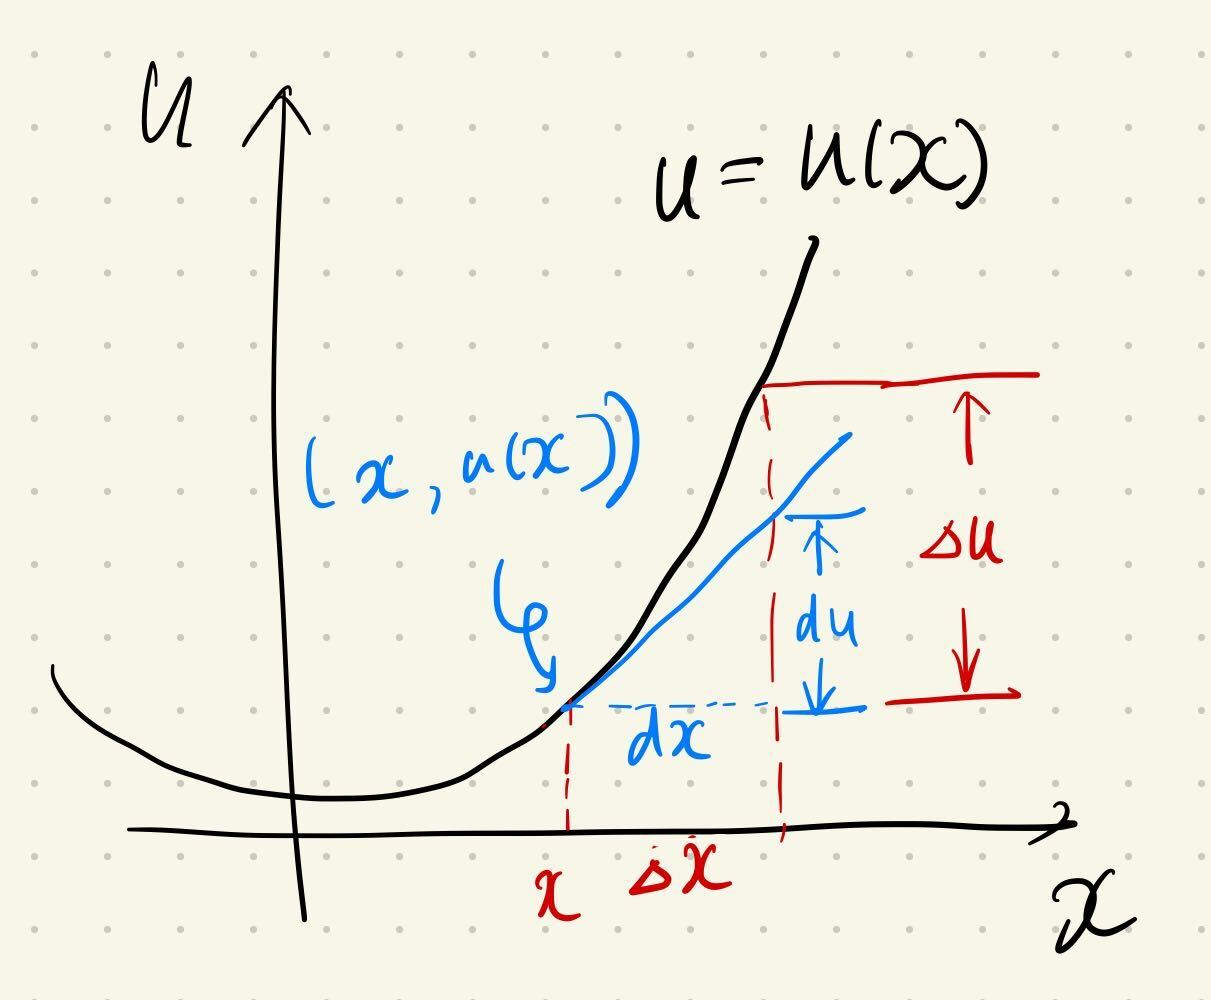
\includegraphics[width = 0.5\textwidth]{figures/chap 06/Differential.png}
\end{figure}

In this virtue, we can treat $du$ and $dx$ as manipulable entities and write
\[du = u'(x)dx\]
For example, say $u(x) = x^2$, then since $u'(x) = 2x$, we have $du = 2xdx$.  In fact, we have implicitly used the concept of differentials before when we we doing linear approximations.  Suppose we would like to approximate $u(x)$ around $x = x_0$, previously we used the tangent line equation and derived the linear approximant
\[\hat{u}(x) = u(x_0) + u'(x_0) (x - x_0)\]
Now with the differential notation, we can write $x = x_0 + dx$ and yield
\[\hat{u}(x) = \hat{u}(x_0 + dx) = u(x_0) + du = u(x_0) + u'(x_0)dx\]

To familiarize ourselves with the differential notation, let us look at a few examples:
\begin{eg}[]{eg: differentials}
    Given following functional relationship between $u$ and $x$, express $du$ with $dx$
    \begin{tasks}(4)
        \task $u = x + 1$
        \task $u = 3x + 2$
        \task $u = x^2 + 1$
        \task $u = \cos x$
        \task $u = x^3 - \sec x$
        \task $x = e^u$
        \task $x = \tan u$
        \task $x = \sin u$
    \end{tasks}
\end{eg}

\begin{egsol}[]{egsol: differentials}
    \begin{enumerate}[a)]
        \item Since $u'(x) = 1$, we have $du = u'(x)dx = dx$.
        \item Since $u'(x) = 3$, we have $du = u'(x)dx = 3dx$.
        \item Since $u'(x) = 2x$, we have $du = u'(x)dx = 2xdx$.
        \item Since $u'(x) = -\sin x$, we have $du = u'(x)dx = -\sin xdx$.
        \item Rewriting $u(x) = x^3 - \frac{1}{\cos x}$, we have $u'(x) = 3x^2 - \big(-\frac{1}{\cos^2 x}\big)\cdot(-\sin x) = 3x^2 - \tan x \sec x$.  Therefore, $du = u'(x)dx = (3x^2 - \tan x \sec x) dx$.
        \item Since $x'(u) = e^u$, we have $dx = x'(u)du = e^u du = x du$.  Therefore, $du = \frac{dx}{x}$.
        \item Since $x'(u) = \sec^2 u$, we have $dx = x'(u)du = \sec^2 u du = (1+\tan^2 u) du = (1+x^2) du$.  Therefore, $du = \frac{dx}{1+x^2}$.
        \item Since $x'(u) = \cos u$, we have $dx = x'(u)du = \cos u du$.  Therefore, $du = \frac{dx}{\cos u}$.  If $u$ is restricted between $-\frac{\pi}{2}$ and $\frac{\pi}{2}$, we can further reduce $\cos u = \sqrt{1-\sin^2 u} = \sqrt{1-x^2}$, so we have $du = \frac{dx}{\sqrt{1-x^2}}$.
    \end{enumerate}
\end{egsol}

\subsection{U-substitution}

Differentials are extremely useful in some types of antidifferentiation problems, since we can make the antidifferentiation tractable after replacing the variable of interest and substituting the differentials.  For example, in the teaser above where we try to fine $\int \frac{x}{\sqrt{x^2+1}} dx$, suppose we let $u = x^2 + 1$, then we have $du = 2xdx$, so we yield
\begin{align*}
    \int \frac{x}{\sqrt{x^2+1}} dx &= \int \frac{1}{2}\frac{2xdx}{\sqrt{x^2+1}}\\
    &= \int \frac{1}{2}\frac{du}{\sqrt{u}}\\
    &= \int \frac{1}{2} u^{-1/2} du\\
    &= \frac{1}{2} \cdot \frac{1}{1/2}u^{1/2} + C = \sqrt{u} + C = \sqrt{x^2+1} + C
\end{align*}
where we need to remember to substitute $u$ back to $x$.  We may check that this substitution trick is valid by differentiating $\sqrt{x^2+1} + C$ with respect to $x$, which gets us back to $\frac{x}{\sqrt{x^2+1}}$. 

This technique is called the \textbf{U-substitution} since in the midst of the derivation, we 
 substituted our original target of antidifferentiation, $x$, with a new variable $u$.  The general form of U-substitution can be written as follows:
\[\int f(u(x)) u'(x) dx = \int f(u) du = F(u) + C = F(u(x)) + C\]
where $F(.)$ is an antiderivative of $f(.)$.  In our example, we had $f(.)$ as the reciprocal of square root, and $u(x) = x^2 + 1$.

The million dollar question is whether we have a standard procedure that finds the appropriate $u(x)$ that makes U-substitution work.  Unfortunately, there isn't a one-size-fit-all solution, and sometimes we'll need some experience, quite a bit of trial and error, and a lot of luck.  However, we can reinspect what we have done above and come up with a general rule of thumb:
\begin{enumerate}
    \item We write out our antidifferentiation problem:
    \[\int \frac{x}{\sqrt{x^2+1}} dx\]
    \item First we inspect the integrand and find a portion in the integrand shaped like a composite function $f(u(x))$, where we \textit{know} the antiderivative of $f(.)$.  In the example above, $f(.)$ is the reciprocal of square root, and $u(x) = x^2 + 1$ is the function within $f(.)$.  
    \[\int \frac{\textcolor{blue}{x}}{\textcolor{red}{\sqrt{\textcolor{orange}{x^2+1}}}} dx = \int \textcolor{red}{\frac{1}{\sqrt{\textcolor{orange}{u}}}} \cdot \textcolor{blue}{x}dx\]
    Up until now we are doing the same thing as chain rule in derivatives, where we also trid to identify composite functions $f(u(x))$ that we know the derivative of $f(.)$.
    \item Right now in the integrand we have a function of $u$ and a remainder of function of $x$. Our goal is that after substituting the differential $dx$ with $du$, the function of $x$ would vanish, leaving us a pure integrand consisting of $u$.  Since $du = u'(x)dx$, the second step is to calculate $u'(x)$ and check that after dividing $u'(x)$ from the remainder of the integrand, \textit{there is no more $x$ left}.  If not, then we will have to go back to the previous step and pick a better $f(u(x))$. In the example above, $u'(x) = (x^2 + 1)' = 2x$, and the remainder of the integrand is $x$, so we have $\frac{x}{2x} = \frac{1}{2}$, which is free of $x$ and greenlights our U-substitution.
    \[\int \textcolor{red}{\frac{1}{\sqrt{\textcolor{orange}{u}}}} \cdot \textcolor{blue}{x} dx = \int \textcolor{red}{\frac{1}{\sqrt{\textcolor{orange}{u}}}} \cdot \textcolor{blue}{x} \textcolor{orange}{\frac{du}{u'(x)}} =\int \textcolor{red}{\frac{1}{\sqrt{\textcolor{orange}{u}}}} \cdot \underbrace{\frac{\textcolor{blue}{x}}{\textcolor{orange}{u'(x)}}}_{\substack{\text{Should not} \\ \text{depend on }x}} \textcolor{orange}{du}\]
    \item After confirming U-substitution may work, perform U-substitution based on the selected $f(.)$ and $u(x)$.
\end{enumerate}

In the following, let's look at some examples utilizing U-substitution.

\begin{eg}[]{eg: u_sub_1}
    Find the following antiderivatives.
    \begin{tasks}(4)
        \task $\int 2x(x^2+1)^3 dx$
        \task $\int 3x^2\sqrt{x^3-2} dx$
        \task $\int x\sqrt[3]{3-4x^2} dx$
        \task $\int \sqrt{1-5x} dx$
        \task $\int \frac{x}{1+4x^2} dx$
        \task $\int xe^{x^2+1} dx$
        \task $\int e^{2x}\sqrt{e^{2x}+1} dx$
        \task $\int x\sin(x^2) dx$ 
    \end{tasks}
\end{eg}

\begin{egsol}[]{egsol: u_sub_1}
    \begin{enumerate}[a)]
        \item The composite function here is pretty straightforward: $x^2+1$ as a whole is raised to the third power, so we may try $f(t) = t^3$ and $u(x) = x^2+1$.  Now since $u'(x) = 2x$ and the remainder of the integrand is $2x$, we have $\frac{2x}{2x} = 1$ which is independent of $x$, meaning that U-substitution may work.  We then have, letting $u = x^2+1$ and thus $du = 2xdx$:
        \begin{align*}
            \int 2x(x^2+1)^3 dx &= \int (x^2+1)^3 2xdx\\
            &= \int u^3 du\\
            &= \frac{1}{4}u^4 + C = \frac{1}{4}(x^2+1)^4 + C
        \end{align*}
        Remember the integration constant and substitution of $u$ back into terms of $x$.
        \item The composite function here looks like $x^3-2$ as a whole taken the square root, so we may try $f(t) = \sqrt{t}$ and $u(x) = x^3 - 2$.  Now since $u'(x) = 3x^2$ and the remainder of the integrand is $3x^2$, we have $\frac{3x^2}{3x^2} = 1$ which is independent of $x$.  We then have, letting $u = x^3 - 2$ and thus $du = 3x^2dx$:
        \begin{align*}
            \int 3x^2\sqrt{x^3-2} dx &= \int (x^3-2)^{1/2} 3x^2dx\\
            &= \int u^{1/2} du\\
            &= \frac{1}{1+1/2}u^{1+1/2} + C = \frac{2}{3}(x^3-2)^{3/2} + C
        \end{align*}
        \item The composite function here looks like $3-4x^2$ as a whole taken the cube root, so we may try $f(t) = \sqrt[3]{t}$ and $u(x) = 3 - 4x^2$.  Now since $u'(x) = -8x$ and the remainder of the integrand is $x$, we have $\frac{x}{-8x} = -\frac{1}{8}$ which is independent of $x$.  We then have, letting $u = 3 - 4x^2$ and thus $du = -8xdx$:
        \begin{align*}
            \int x\sqrt[3]{3-4x^2} dx &= -\frac{1}{8}\int (3-4x^2)^{1/3} (-8x)dx\\
            &= -\frac{1}{8}\int u^{1/3} du\\
            &= -\frac{1}{8}\cdot\frac{1}{1+1/3}u^{1+1/3} + C \\
            &= -\frac{1}{8}\cdot\frac{3}{4}u^{4/3} + C = -\frac{3}{32}(3-4x^2)^{4/3} + C
        \end{align*}
        Note that here after substituting the differentials, we yield an additional factor $-\frac{1}{8}$.
        \item The composite function here looks like $1-5x$ as a whole taken the square root, so we may try $f(t) = \sqrt{t}$ and $u(x) = 1-5x$.  Now since $u'(x) = -5$ and the remainder of the integrand is $1$, we have $\frac{1}{-5} = -\frac{1}{5}$ which is independent of $x$.  We then have, letting $u = 1-5x$ and thus $du = -5dx$:
        \begin{align*}
            \int \sqrt{1-5x} dx &= -\frac{1}{5}\int (1-5x)^{1/2} (-5)dx\\
            &= -\frac{1}{5}\int u^{1/2} du\\
            &= -\frac{1}{5}\cdot\frac{1}{1+1/2}u^{1+1/2} + C \\
            &= -\frac{1}{5}\cdot\frac{2}{3}u^{3/2} + C = -\frac{2}{15}(1-5x)^{3/2} + C
        \end{align*}
        \item The composite function here looks like $1+4x^2$ as a whole taken the reciprocal, so we may try $f(t) = \frac{1}{t}$ and $u(x) = 1+4x^2$.  Now since $u'(x) = 8x$ and the remainder of the integrand is $x$, we have $\frac{x}{8x} = \frac{1}{8}$ which is independent of $x$.  We then have, letting $u = 1+4x^2$ and thus $du = 8xdx$:
        \begin{align*}
            \int \frac{x}{1+4x^2} dx &= \frac{1}{8}\int  \frac{1}{1+4x^2} 8xdx\\
            &= \frac{1}{8}\int \frac{1}{u} du\\
            &= \frac{1}{8}\ln |u| + C = \frac{1}{8} \ln |1+4x^2| + C
        \end{align*}
        \item The composite function here looks like $x^2+1$ as a whole taken the exponential, so we may try $f(t) = e^t$ and $u(x) = x^2+1$.  Now since $u'(x) = 2x$ and the remainder of the integrand is $x$, we have $\frac{x}{2x} = \frac{1}{2}$ which is independent of $x$.  We then have, letting $u = x^2 + 1$ and thus $du = 2xdx$:
        \begin{align*}
            \int xe^{x^2+1} dx &= \frac{1}{2}\int e^{x^2+1} 2xdx\\
            &= \frac{1}{2}\int e^u du\\
            &= \frac{1}{2} e^u + C = \frac{1}{2} e^{x^2+1} + C
        \end{align*}
        \item The composite function here looks like $e^{2x}+1$ as a whole taken the square root, so we may try $f(t) = \sqrt{t}$ and $u(x) = e^{2x}+1$.  Now since $u'(x) = 2e^{2x}$ and the remainder of the integrand is $e^{2x}$, we have $\frac{e^{2x}}{2e^{2x}} = \frac{1}{2}$ which is independent of $x$.  We then have, letting $u = e^{2x} + 1$ and thus $du = 2e^{2x}dx$:
        \begin{align*}
            \int e^{2x}\sqrt{e^{2x}+1} dx &= \frac{1}{2}\int (e^{2x}+1)^{1/2} 2e^{2x}dx\\
            &= \frac{1}{2}\int u^{1/2} du\\
            &= \frac{1}{2}\cdot\frac{1}{1+1/2} u^{1+1/2} \\
            &= \frac{1}{2}\cdot\frac{2}{3} u^{3/2} + C = \frac{1}{3} (e^{2x}+1)^{3/2} + C
        \end{align*}
        \item The composite function here looks like $x^2$ as a whole taken the sine function, so we may try $f(t) = \sin t$ and $u(x) = x^2$.  Now since $u'(x) = 2x$ and the remainder of the integrand is $x$, we have $\frac{x}{2x} = \frac{1}{2}$ which is independent of $x$.  We then have, letting $u = x^2$ and thus $du = 2xdx$:
        \begin{align*}
            \int x \sin(x^2) dx &= \frac{1}{2}\int \sin(x^2) 2xdx\\
            &= \frac{1}{2}\int \sin u du\\
            &= \frac{1}{2} (-\cos u) + C = -\frac{1}{2} \cos(x^2) + C
        \end{align*}
    \end{enumerate}
\end{egsol}

\begin{ex}[]{ex: u_sub_1}
    Find the following antiderivatives.
    \begin{tasks}(3)
        \task $\int (1-\frac{1}{x}) \cos (x - \ln x) dx$
        \task $\int \sin x \cos x dx$
        \task $\int \sin(2x) (1 - \cos(2x))^3 dx$
        \task $\int \frac{2}{3x + 1} dx$
        \task $\int \frac{2x}{3x^2 + 1} dx$
        \task $\int \frac{2}{3x^2 + 1} dx$
        \task $\int \frac{x^2 + 1}{x^3 + 3x} dx$
        \task $\int \frac{x}{\sqrt{1-x^2}} dx$ 
        \task $\int \tan x dx$ 
    \end{tasks}
\end{ex}

 \begin{exsol}[]{exsol: u_sub_1}
    \begin{enumerate}[a)]
        \item The composite function here is pretty straightforward: $x - \ln x$ as a whole is taken the cosine function, so we may try $f(t) = \cos t$ and $u(x) = x - \ln x$.  Now since $u'(x) = 1 - \frac{1}{x}$ and the remainder of the integrand is exactly the same, we conclude that U-substitution may work.  We then have, letting $u = x - \ln x$ and thus $du = \big(1-\frac{1}{x}\big)dx$:
        \begin{align*}
            \int \Big(1-\frac{1}{x}\Big) \cos(x - \ln x) dx &= \int \cos(x - \ln x) \Big(1-\frac{1}{x}\Big)dx\\
            &= \int \cos u du\\
            &= \sin u + C = \sin(x - \ln x) + C
        \end{align*}
        \item Here we do not have an evident composite function, but we can let $f(t) = 1$ and $u(x) = \sin x$.  Then, the remaining integrand is $\cos x$, which is exactly $u'(x)$, so the U-substitution may work.  Letting $u = \sin x$ and thus $du = \cos x dx$ and we have:
        \[\int \sin x \cos x dx = \int u du = \frac{1}{2} u^2 + C = \frac{1}{2} \sin^2x + C\]
        Alternatively, we may let $u(x) = \cos x$ so that the remaining integrand is $\sin x$, which is equal to $-u'(x)$ so the U-substitution may still work.  Letting $u = \cos x$ and thus $du = -\sin x dx$ and we have:
        \[\int \sin x \cos x dx = -\int \cos x (-\sin x)dx = -\int u du = -\frac{1}{2} u^2 + C = -\frac{1}{2} \cos^2x + C\]
        Still another way is to recall that $\sin 2x = 2\sin x \cos x$, so we have, letting $u = 2x$ so that $du = 2dx$:
        \begin{align*}
            \int \sin x \cos x dx &= \frac{1}{2}\int 2 \sin x \cos x dx\\
            &= \frac{1}{2} \int \sin(2x) dx\\
            &= \frac{1}{4} \int \sin(2x) \cdot 2dx\\
            &= \frac{1}{4} \int \sin u du = \frac{1}{4} (- \cos u) + C = -\frac{1}{4}\cos 2x + C
        \end{align*}
        At first glance, it seems that the three methods are giving us different answers.  However, we can use two identities, $\sin^2 x + \cos^2 x = 1$ and $\cos 2x = 2 \cos^2x - 1$ to show that
        \begin{gather*}
            \frac{1}{2}\sin^2x + C = \frac{1}{2}(1-\cos^2x) + C = -\frac{1}{2}\cos^2x + \Big(C+\frac{1}{2}\Big)\\
            -\frac{1}{4}\cos 2x + C  = -\frac{1}{4}(2 \cos^2 x - 1) + C = -\frac{1}{2}\cos^2x + \Big(C+\frac{1}{4}\Big)
        \end{gather*}
        Since $C$ is any constant, we may redefine $C$ for the first and third method, then their answers would match the $-\frac{1}{2}\cos^2x + C$ solution.  That is, these three answers are \textit{de facto} equivalent.
        \item Here if we just let $u(x) = 2x$, then it would work since we still don't have a quick idea on how to antidifferentiate $\sin u (1- \cos u)^3$.  However, we can try letting $f(t) = t^3$ and $u(x) = 1-\cos (2x)$.  Now since $u'(x) = 2\sin(2x)$, which is twice the remainder, $\sin (2x)$, the U-substitution should work now.  We then have, letting $u = 1-\cos (2x)$ and thus $du = 2\sin (2x)dx$
        \begin{align*}
            \int \sin(2x)(1-\cos(2x))^3 dx &= \frac{1}{2}\int (1-\cos(2x))^3 2\sin(2x) dx\\
            &= \frac{1}{2}\int u^3 du\\
            &= \frac{1}{2}\cdot\frac{1}{4}u^{4} + C = \frac{1}{8}(1-\cos (2x))^4 + C
        \end{align*}
        \item The composite function here looks like $3x+1$ as a whole taken the reciprocal, so we may try $f(t) = \frac{1}{t}$ and $u(x) = 3x+1$.  Now since $u'(x) = 3$ and the remainder of the integrand is $2$, we have $\frac{2}{3}$ is independent of $x$ and U-substitution should work.  We then have, letting $u = 3x+1$ and thus $du = 3dx$:
        \begin{align*}
            \int \frac{2}{3x+1} dx &= \frac{2}{3}\int \frac{1}{3x+1} 3dx\\
            &= \frac{2}{3}\int \frac{1}{u} du\\
            &= \frac{2}{3}\ln |u| + C = \frac{2}{3} \ln |3x+1| + C
        \end{align*}
        \item The composite function here looks like $3x^2 +1$ as a whole taken the reciprocal, so we may try $f(t) = \frac{1}{t}$ and $u(x) = 3x^2 + 1$.  Now since $u'(x) = 6x$ and the remainder of the integrand is $2x$, we have $\frac{2x}{6x} = \frac{1}{3}$ which is independent of $x$.  We then have, letting $u = 3x^2 + 1$ and thus $du = 6xdx$:
        \begin{align*}
            \int \frac{2x}{3x^2 + 1} dx &= \frac{1}{3}\int \frac{1}{3x^2 + 1} 6xdx\\
            &= \frac{1}{3}\int \frac{1}{u} du\\
            &= \frac{1}{3}\ln |u| + C = \frac{1}{3} \ln |3x^2 + 1| + C
        \end{align*}
        \item Here if we still let $f(t) = \frac{1}{t}$ and $u(x) = 3x^2+1$, we would fail since  $u'(x) = 6x$ and the remainder of the integrand is $2$, and we have $\frac{2}{6x} = \frac{1}{3x}$ which is dependent of $x$.  On closer inspection, we can rewrite the integrand as:
        \[\frac{2}{3x^2+1} = \frac{2}{(\sqrt{3}x)^2 + 1}\]
        The denominator now has the shape of $\frac{1}{1+t^2}$, which reminds us of the arctangent function.  Therefore, letting $f(t) = \frac{1}{1+t^2}$ and $u(x) = \sqrt{3}x$, we have $u'(x) = \sqrt{3}$ and the integrand remainder $2$ are both constants, so the U-substitution should work.  We then have, letting $u = \sqrt{3}x$ and thus $du = \sqrt{3}dx$:
        \begin{align*}
            \int \frac{2}{3x^2+1} dx &= \frac{2}{\sqrt{3}}\int \frac{1}{(\sqrt{3}x)^2 + 1} \sqrt{3}dx\\
            &= \frac{2}{\sqrt{3}}\int \frac{1}{1+u^2} du\\
            &= \frac{2}{\sqrt{3}} \arctan u + C = \frac{2}{\sqrt{3}} \arctan(\sqrt{3}x) + C
        \end{align*}
        \item The composite function here looks like $x^3+3x$ as a whole taken the reciprocal, so we may try $f(t) = \frac{1}{t}$ and $u(x) = x^3+3x$.  Now since $u'(x) = 3x^2+3$ and the remainder of the integrand is $x^2+1$, we have $\frac{x^2+1}{x^3+3x} = \frac{1}{3}$ which is independent of $x$.  We then have, letting $u = x^3 + 3x$ and thus $du = 3(x^2 + 1)dx$:
        \begin{align*}
            \int \frac{x^2+1}{x^3+3x} dx &= \frac{1}{3}\int \frac{1}{x^3+3x} 3(x^2+1)dx\\
            &= \frac{1}{3}\int \frac{1}{u} du\\
            &= \frac{1}{3} \ln |u| + C = \frac{1}{2} \ln|x^3+3x| + C
        \end{align*}
        \item The composite function here looks like $1-x^2$ as a whole taken the reciprocal of square root, so we may try $f(t) = \frac{1}{\sqrt{t}}$ and $u(x) = 1-x^2$.  Now since $u'(x) = -2x$ and the remainder of the integrand is $x$, we have $\frac{x}{-2x} = -\frac{1}{2}$ which is independent of $x$.  We then have, letting $u = 1-x^2$ and thus $du = -2xdx$:
        \begin{align*}
            \int \frac{x}{\sqrt{1-x^2}} dx &= -\frac{1}{2}\int (1-x^2)^{-1/2} (-2x)dx\\
            &= -\frac{1}{2}\int u^{-1/2} du\\
            &= -\frac{1}{2} \cdot \frac{1}{1-1/2} u^{1-1/2} + C \\
            &= -\frac{1}{2} \cdot 2 u^{1/2} + C = -sqrt{1-x^2} + C
        \end{align*}
        \item At first glance there it looks like we do not have any idea on what to substitute as $u$.  However, if we rewrite the integrand as:
        \[\tan x = \frac{\sin x}{\cos x}\]
        We can see that setting $f(t)= \frac{1}{t}$ and $u(x) = \cos x$ would lead to $u'(x) = -\sin x$, whose multiple appears in the numerator as the remainder of the integrand.  Therefore, her we let $u = \cos x$ and thus $du = -\sin x$:
        \begin{align*}
            \int \tan x dx &= \int \frac{\sin x}{\cos x} dx\\
            &= -\int \frac{1}{\cos x} (-\sin x)dx\\
            &= -\int \frac{1}{u} du\\
            &= -\ln |u| + C = -\ln|\cos x| + C
        \end{align*}
        Or, alternatively, we may write
        \begin{equation*}
            -\ln |\cos x| + C = \ln |\cos x|^{-1} + C= \ln \frac{1}{|\cos x|} + C = \ln \Big|\frac{1}{\cos x}\Big| + C = \ln |\sec x| + C
        \end{equation*}
    \end{enumerate}
\end{exsol}
After we have mastered how U-substitution works, sometimes we can look at the integrand and plan out how the substitution would work, without writing explicitly what $f(.)$ and the integrand remainder would be.  Here we try a couple of antidifferentiation variants that can still use U-substitution, albeit with a little twist:
\begin{eg}[]{eg: u_sub_2}
    Find the following antiderivatives.
    \begin{tasks}(3)
        \task $\int \sin x(4\cos^3 x$\\ $- 3\cos^2x + 2) dx$
        \task $\int \frac{1}{1+x} + \sin(1-x) dx$
        \task $\int \frac{3}{x^2+4} dx$
        \task $\int \frac{2x+3}{x^2+4} dx$
        \task $\int \frac{1}{x \ln x} dx$
        \task $\int 2x^3\sqrt{x^2+1} dx$
    \end{tasks}
\end{eg}
\begin{egsol}[]{egsol: u_sub_2}
    \begin{enumerate}[a)]
        \item Here it would be intuitive to set $u = \cos x$, since $du = -\sin x dx$ and $\sin x$ appears in the front.  Therefore, we have
        \begin{align*}
            \int \sin x(4\cos^3 x - 3\cos^2 x + 2) dx &= -\int (4\cos^3 x - 3\cos^2x + 2) (-\sin x)dx\\
            &= -\int (4u^3-3u^2+2) du\\
            &= -(u^4-u^3+2u) + C = -\cos^4x + \cos^3x - 2\cos x + C
        \end{align*}
        \item Here if we directly substitute $u = 1-x$ for the latter term, the first term would become $\frac{1}{2-u}$ and still be intractable.  Therefore, we should split the integrand first with the sum rule:
        \[\int \frac{1}{1+x} + \sin(1-x) dx = \int \frac{1}{1+x} dx + \int \sin(1-x) dx\]
        Then we can try to substitute $u = 1+x$ ($du = dx$) for the first term and $v = 1-x$ ($dv = -dx$) for the second term:
        \begin{align*}
            \int \frac{1}{1+x} dx + \int \sin(1-x) dx &= \int \frac{1}{1+x} dx - \int \sin(1-x) (-dx)\\
            &= \int \frac{1}{u} du - \int \sin v dv\\
            &= \ln |u| - (-\cos v) + C = \ln |1+x| + \cos(1-x) + C
        \end{align*}
        \item Here the intuition would be to set $u(x) = x^2 + 4$.  However, in this case since $u'(x) = 2x$, we would need a multiple of $x$ in the integrand to make up $u'(x)dx = 2xdx$, so this substitution would not work.  Here the way to go through is to rewrite the integrand as:
        \[\int \frac{3}{x^2+4} dx = \int \frac{3}{4}\frac{1}{\frac{x^2}{4} + 1} dx = \int \frac{3}{4}\frac{1}{\big(\frac{x}{2}\big)^2 + 1} dx\]
        Now the integrand has the form $\frac{1}{u^2+1}$, which prompts us to do a substitution of $u=\frac{x}{2}$ and thus $du = \frac{1}{2}dx$, leading to:
        \begin{align*}
            \int \frac{3}{4}\frac{1}{\big(\frac{x}{2}\big)^2 + 1} dx &= \frac{3}{2} \int \frac{1}{\big(\frac{x}{2}\big)^2 + 1} \frac{1}{2}dx\\
            &= \frac{3}{2}\int \frac{1}{u^2+1} du\\
            &= \frac{3}{2} \arctan u + C = \frac{3}{2} \arctan\big(\frac{x}{2}\big) + C
        \end{align*}
        \item Here if we set $u(x) = x^2 + 4$, then $u'(x) = 2x$, which partially appears in the numerator, but the numerator is still not a multiple of $2x$.  Yet note that we can split the integrand first as:
        \[\int \frac{2x+3}{x^2+4} dx = \int \frac{2x}{x^2+4} dx + \int \frac{3}{x^2+4} dx\]
        Now the first antiderivative term can be found with U-substitution of $u(x) = x^2 + 4$ since the numerator is now just $2x = u'(x)$.  For the second term, our experience in the previous subproblem prompts us to do another rewriting of the integrand:
        \[\int \frac{2x}{x^2+4} dx + \int \frac{3}{x^2+4} dx= \int \frac{2x}{x^2+4} dx+ \int\frac{3}{4}\cdot\frac{1}{\big(\frac{x}{2}\big)^2+1}dx\]
        so that we can do another substitution with $v = \frac{x}{2}$ and $dv = \frac{1}{2}dx$.  Now we have,
        \begin{align*}
            \int \frac{2x}{x^2+4} dx+ \int\frac{3}{4}\cdot\frac{1}{\big(\frac{x}{2}\big)^2+1}dx &= \int \frac{1}{x^2+4} \cdot 2xdx+ \frac{3}{2}\int\frac{1}{\big(\frac{x}{2}\big)^2+1} \cdot \frac{1}{2}dx\\
            &= \int \frac{1}{u} du + \frac{3}{2}\int\frac{1}{v^2+1}dv\\
            &= \ln |u| + \frac{3}{2}\arctan v + C\\
            &= \ln |x^2 + 4| + \frac{3}{2} \arctan\big(\frac{x}{2}\big) + C
        \end{align*}
        \item Here since $\frac{d}{dx} \ln x = \frac{1}{x}$, it prompts us to let $u = \ln x$ and $du = \frac{1}{x} dx$, so we have
        \begin{align*}
            \int \frac{1}{x \ln x} dx &= \int \frac{1}{\ln x} \cdot \frac{1}{x}dx\\
            &= \int \frac{1}{u} du\\
            &= \ln |u| + C = \ln |\ln x| + C
        \end{align*}
        \item Here the natural choice of $u$ would be $u = x^2+1$, which leads to $du = 2xdx$.  Therefore, at first glance U-substitution would fail since the remainder of the integrand is $2x^3$ instead of a constant multiple of $2x$.  However, note if we follow through, using the identity $x^2 = u - 1$:
        \begin{align*}
            \int 2x^3 \sqrt{x^2 + 1}dx &= \int x^2 (x^2+1)^{1/2} \cdot 2xdx\\
            &= \int (u-1) u^{1/2} du\\
            &= \int u^{3/2} - u^{1/2} du\\
            &= \frac{2}{5}u^{5/2} - \frac{2}{3}u^{3/2} + C = \frac{2}{5}(x^2+1)^{5/2} - \frac{2}{3}(x^2+1)^{3/2} + C
        \end{align*}
    \end{enumerate}
\end{egsol}
All in all, U-substitution is a very versatile technique that can aid us in finding antiderivatives.  However, this requires us to sometimes pretreat the integrand and also identify the correct $u(x)$.  Therefore, successful application of U-substitution would require some experience, which can only be obtained by repeated exercises.

\subsection{Interlude: Products between Trigonometric Functions}
Now we have mastered the technique of U-substitution, we can solve a particular type of antidifferentiation that comes up fairly frequently, which is the the product of powers of trigonometric.  Specifically in the course, we are looking for the following type of antiderivative:
\[\int \sin^m x \cos^n x~dx,  m \in \mathbb{N}, n \in \mathbb{N}\]
As we will see, this type of antiderivative can be tackled with carefully performed U-substitution, and sometime with the help of the following three trigonometric identities:
\begin{gather*}
    \sin^2 x + \cos^2 x = 1\\
    \cos^2 x = \frac{1+\cos 2x}{2}\\
    \sin^2 x = \frac{1-\cos 2x}{2}
\end{gather*}
where the second and third identity come from the double angle formula for cosines.  Let's first look at the following antiderivatives as a warm-up:
\begin{eg}[]{eg: trig_1_2}
Find the following antiderivative:
\[\int \sin x \cos^2 x~dx\]
\end{eg}
\begin{egsol}[]{egsol: trig_1_2}
    Here it would be intuitive to let $u(x) = \cos x$, since the remainder of the integrand after the U-substitution would be $\sin x$, which can be taken care of by $du = -\sin x dx$.  To spell it out:
\begin{equation*}
    \int \sin x \cos^2 x~dx = -\int \cos^2 x (-\sin x~dx) = -\int u^2~du = -\frac{1}{3}u^3 + C = -\frac{1}{3}\cos^3 x + C
\end{equation*}
    Note that if we let $u(x) = \sin x$, then the remainder of the integrand after substitution would be $\cos^2 x$, which does not fit $du = \cos x dx$, so this substitution thus does not work.
\end{egsol}
\begin{ex}[]{ex: trig_4_1}
Find the following antiderivative:
\[\int \sin^4 x \cos x~dx\]
\end{ex}
\begin{exsol}[]{eg: trig_4_1}
    Here instead we would need to let $u(x) = \sin x$, so that the remainder of the integrand after the U-substitution would be $\cos x$, which is then taken care of by $du = \cos x dx$.  That is:
\begin{equation*}
    \int \sin^4 x \cos x~dx = \int \sin^4 x (\cos x~dx) = \int u^4~du = \frac{1}{5}u^5 + C = \frac{1}{5}\sin^5 x + C
\end{equation*}
    Note that if we let $u(x) = \cos x$, then the remainder of the integrand after substitution would be $\sin^4 x$, which does not fit $du = -\sin x dx$, so this substitution thus does not work.
\end{exsol}
From the examples above, we can see that since $d (\sin x) = \cos x~dx$ and $d (\cos x) = -\sin x~dx$, in the case where one of the trigonometric functions has power of $1$, we can set \textit{the other} trigonometric function as $u(x)$, then substitution of differentials will take care of the remaining integrand and we're done.  With this technique in hand, we can now actually antidifferentiate any case with either $m$ or $n$ as odd number using the identity $\sin^2 x + \cos^2x = 1$.  To see this, let's look at the following examples:
\begin{eg}[]{eg: trig_3_2}
Find the following antiderivative:
\[\int \sin^3 x \cos^2 x~dx\]
\end{eg}
\begin{egsol}[]{egsol: trig_3_2}
    At face value, it seems that both letting $u(x)=\sin x$ and $u(x)=\cos x$ do not eliminate the remainder in the integrand.  However, if we use the identity $\sin^2 x + \cos^2 x = 1- \cos^2 x$ and replace $\sin^2 x$ with $(1 - \cos^2 x)$, we yield:
    \[\int \sin^3 x \cos^2x~dx = \int \sin x (\sin^2 x) \cos^2 x~dx = \int \sin x (1 - \cos^2 x) \cos^2 x~dx\]
    Now $\sin x$ has a power of $1$, so the problem is reduced to the case in the previous two examples: we just need to let $u(x) = \cos x$, so that $du = -\sin x dx$ and
    \begin{align*}
        \int \sin x (1 - \cos^2 x) \cos^2 x~dx &= -\int (1-\cos^2 x) \cos^2 x (-\sin x~dx)\\
        &= -\int (1-u^2)u^2~du\\
        &= -\int u^2~du + \int u^4~du\\
        &= -\frac{1}{3}u^3 + \frac{1}{5}u^5 + C = -\frac{1}{3}\cos^3 x + \frac{1}{5} \cos^5 x + C
    \end{align*}
    Note that if we instead tried to substitute $\cos^2 x$ with $(1-\sin^2 x)$, the following U-substitution would not work.  To see this, after the substitution we will get
    \[\int \sin^3 x \cos^2x~dx = \int \sin^3 x (1-\sin^2 x)~dx\]
    which does not have $\cos x$ in the integrand.  However, if we let $u(x) = \sin x$, we have $du = \cos x~dx$ so we \textit{need} a $\cos x$ in the integrand.  This line of U-substitution therefore fails.
\end{egsol}
\begin{ex}[]{ex: trig_one_odd}
Find the following antiderivatives:
    \begin{tasks}(3)
        \task $\int \sin^4 x \cos^3 x~dx$
        \task $\int \sin^5 x \cos^2 x~dx$
        \task $\int \sin^3 x \cos^3 x~dx$
    \end{tasks}
\end{ex}
\begin{exsol}[]{exsol: trig_one_odd}
    \begin{enumerate}[a)]
        \item Here since the power of $\cos x$ is odd, we opt to substitute $\cos^2 x$ with $(1-\sin^2 x)$ so that after the substitution, we would have one $\cos x$ left for U-substitution to work.  Namely,
        \[\int \sin^4 x \cos^3 x~dx = \int \sin^4 x \cos^2x \cos x~dx = \int \sin^4 x (1-\sin^2 x) \cos x~dx\]
        Let $u(x) = \sin x$ so that $du = \cos x~dx$, and we have
        \begin{align*}
            \int \sin^4 x (1-\sin^2 x) \cos x~dx &= \int u^4 (1-u^2) du\\
            &= \int (u^4 - u^6) du\\
            &= \frac{1}{5}u^5 - \frac{1}{7}u^7 + C = \frac{1}{5}\sin^5 x - \frac{1}{7}\sin^7 x + C
        \end{align*}
        \item Here since the power of $\sin x$ is odd, we substitute $\sin^4 x$ with $(1-\cos^2 x)^2$ so that after the substitution, we would have on $\sin x$ left for U-substitution to work.  In detail,
        \[\int \sin^5 x \cos^2 x~dx = \int \sin^4 x \cos^2x \sin x~dx = \int (1-\cos^2x)^2 \cos^2x \sin x~dx\]
        Let $u(x) = \cos x$ so that $du = -\sin x~dx$, and we have
        \begin{align*}
            \int (1-\cos^2x)^2 \cos^2x \sin x~dx &= -\int (1-\cos^2x)^2 \cos^2x (-\sin x~dx)\\
            &= -\int (1 - u^2)^2 u^2 du\\
            &= -\int (1 - 2u^2 + u^4)u^2 du\\
            &= -\int (u^2 - 2u^4 + u^6) du\\
            &= -\frac{1}{3}u^3 + \frac{2}{5}u^5 - \frac{1}{7}u^7 + C = -\frac{1}{3}\cos^3x + \frac{2}{5}\cos^5x - \frac{1}{7}\cos^7x + C
        \end{align*}
        \item In this case, both the powers of $\sin x$ and $\cos x$ are odd, so we may choose to either substitute $\sin^2x$ with $(1-\cos^2x)$ or substitute $\cos^2x$ with $(1-\sin^2x)$.\\
        We first substitute $\sin^2x$ with $(1-\cos^2x)$ and yield:
        \[\int \sin^3 x \cos^3 x~dx = \int \sin^2x \cos^3x \sin x~dx = \int (1-\cos^2x)\cos^3x \sin x~dx\]
        Let $u(x) = \cos x$ so that $du = -\sin x~dx$, and we have
        \begin{align*}
            \int (1-\cos^2x) \cos^3x \sin x~dx &= -\int (1-\cos^2x) \cos^3x (-\sin x~dx)\\
            &= -\int (1 - u^2) u^3 du\\
            &= -\int (u^3 - u^5) du\\
            &= -\frac{1}{4}u^4 + \frac{1}{6}u^6 + C = -\frac{1}{4}\cos^4x + \frac{1}{6}\cos^6x + C
        \end{align*}
        Alternatively, we can substitute $\cos^2x$ with $(1-\sin^2x)$ and yield:
        \[\int \sin^3 x \cos^3 x~dx = \int \sin^3x \cos^2x \cos x~dx = \int \sin^3x (1-\sin^2x) \cos x~dx\]
        Let $u(x) = \sin x$ so that $du = \cos x~dx$, and we have
        \begin{align*}
            \int \sin^3x (1-\sin^2x) \cos x~dx &= \int u^3 (1-u^2)du\\
            &= \int (u^3 - u^5) du\\
            &= \frac{1}{4}u^4 - \frac{1}{6}u^6 + C = \frac{1}{4}\sin^4x - \frac{1}{6}\sin^6x + C
        \end{align*}
        At first glance, these two approaches do not seem to arrive at the same answer.  However, we can manipulate the former one as follows:
        \begin{align*}
            -\frac{1}{4}\cos^4x + \frac{1}{6}\cos^6x + C &= -\frac{1}{4}(\cos^2x)^2 + \frac{1}{6}(\cos^2x)^3 + C \\
            &= -\frac{1}{4}(1-\sin^2x)^2 + \frac{1}{6}(1-\sin^2x)^3 + C\\
            &= -\frac{1}{4}(1-2\sin^2x + \sin^4x) + \frac{1}{6}(1-3\sin^2x+3\sin^4x-\sin^6x) + C\\
            &= -\frac{1}{4} + \frac{1}{2} \sin^2x - \frac{1}{4} \sin^4x + \frac{1}{6} -\frac{1}{2}\sin^2x +\frac{1}{2}\sin^4x - \frac{1}{6}\sin^6x + C \\
            &= \frac{1}{4}\sin^4x - \frac{1}{6}\sin^6x + \Big(C - \frac{1}{12}\Big)
        \end{align*}
        Therefore, the two expressions actually imply the same set of antiderivatives since $C$ is just an arbitrary integration constant.
    \end{enumerate}
\end{exsol}
From the examples above, we see that in $\int \sin^mx \cos^nx~dx$ where either $m$ or $n$ is odd, we can use the identity $\sin^2x+\cos^2x = 1$ to reduce the odd-powered trigonometric function to a power of $1$, then use U-substituion as desired.  The only problem left is when both $m$ and $n$ are even, which we will see in the next example. 
\begin{eg}[]{eg: trig_2_2}
Find the following antiderivative:
\[\int \sin^2 x \cos^2 x~dx\]
\end{eg}
\begin{egsol}[]{egsol: trig_2_2}
    Here since both powers are even, substitution between $\sin^2x$ and $\cos^2x$ will never give us a power-$1$ remainder of $\sin x$ or $\cos x$.  One way out is to use the double angle identities we mentioned in the beginning of this subsection.  We substitute $\cos^2x$ with $\frac{1+\cos 2x}{2}$ and $\sin^2x$ with $\frac{1-\sin 2x}{2}$ and yield:
    \begin{equation*}
        \int \sin^2x \cos^2x~dx = \int \frac{1+\cos 2x}{2}\frac{1-\cos 2x}{2}~dx = \frac{1}{4}\int (1-\cos^2 2x) dx
    \end{equation*}
    The second term in the integrand is still a even-powered product of trigonometric functions ($m = 0, n = 2$), so we apply the double angle identity again, now substituting $\cos^2 2x$ with $\frac{1+\cos 4x}{2}$:
    \[\frac{1}{4}\int (1-\cos^2 2x) dx = \frac{1}{4}\int \Big(1-\frac{1+\cos 4x}{2}\Big)~dx = \frac{1}{8}\int (1-\cos 4x)~dx\]
    Now we can finally let $u(x) = 4x$ so that $du = 4 dx$ and yield
    \begin{align*}
        \frac{1}{8}\int (1-\cos 4x)~dx &= \frac{1}{32}\int (1-\cos 4x)(4dx)\\
        &= \frac{1}{32}\int (1-\cos u)~du \\
        &= \frac{1}{32}(u-\sin u) + C = \frac{1}{8}x - \frac{1}{32}\sin 4x + C
    \end{align*}
\end{egsol}
In this example, we see that each time we use the double angle identity, the power of the trigonometric functions will be cut in half.  Therefore, as long as we repeatedly use the double angle identities when we see even powers, the power will eventually be reduced to an odd number, under which we can derive the antiderivative using the techniques we have developed earlier.
\begin{ex}[]{ex: trig_all_even}
Find the following antiderivatives:
    \begin{tasks}(3)
        \task $\int \sin^2x~dx$
        \task $\int \cos^4x~dx$
        \task $\int \sin^4x \cos^2x~dx$
    \end{tasks}
\end{ex}
\begin{exsol}[]{exsol: trig_all_even}
    \begin{enumerate}[a)]
        \item Here we want to find the antiderivative of a even-powered sine / cosine function, so we start with the double angle identity and yield
        \[\int \sin^2x~dx = \int \frac{1-\cos 2x}{2}~dx = \frac{1}{2}\int (1-\cos 2x)~dx\]
        Now we can let $u(x) = 2x$, so that $du = 2dx$ and we have
        \begin{align*}
            \frac{1}{2}\int (1-\cos 2x)~dx &= \frac{1}{4}\int (1-\cos 2x) (2dx)\\
            &= \frac{1}{4}\int (1-\cos u) du\\
            &= \frac{1}{4}(u-\sin u) + C = \frac{1}{2}x - \frac{1}{4} \sin 2x + C
        \end{align*}
        \item This antiderivative also has an integrand of even-powered sine / cosine function, so we still start with the double angle identity and yield
        \begin{align*}
            \int \cos^4x~dx &= \int (\cos^2x)^2 dx\\
            &= \int \Big(\frac{1 + \cos 2x}{2}\Big)^2~dx\\
            &= \frac{1}{4}\int (1 + 2\cos 2x + \cos^2 2x)~dx \\
            &= \frac{1}{4}\int dx + \frac{1}{2}\int \cos 2x~dx + \frac{1}{4}\int \cos^2 2x~dx
        \end{align*}
        The third term in still an even-powered sine / cosine function, so we apply the double angle identity again
        \begin{align*}
            &\frac{1}{4}\int dx + \frac{1}{2}\int \cos 2x~dx + \frac{1}{4}\int \cos^2 2x~dx\\
            = &\frac{1}{4}\int dx + \frac{1}{2}\int \cos 2x~dx + \frac{1}{4}\int \frac{1 + \cos 4x}{2}dx\\
            = &\frac{1}{4}\int dx + \frac{1}{2}\int \cos 2x~dx + \frac{1}{8}\int (1+\cos 4x)~dx
        \end{align*}
        Now we can let $u(x) = 2x, du = 2dx$ and $v(x) = 4x, dv = 4dx$,
        \begin{align*}
            &\frac{1}{4}\int dx + \frac{1}{2}\int \cos 2x~dx + \frac{1}{8}\int (1+\cos 4x)~dx\\
            =&\frac{1}{4}\int dx + \frac{1}{4}\int \cos 2x(2dx) + \frac{1}{32}\int (1+\cos 4x)(4dx)\\
            =&\frac{1}{4}\int dx + \frac{1}{4}\int \cos u~du + \frac{1}{32}\int (1+\cos v) dv\\
            =&\frac{1}{4}x + \frac{1}{4} \sin u + \frac{1}{32}(v + \sin v) + C\\
            =&\frac{1}{4}x + \frac{1}{4} \sin 2x + \frac{1}{32}(4x + \sin 4x) + C\\
            =&\frac{3}{8}x + \frac{1}{4} \sin 2x + \frac{1}{32} \sin 4x + C
        \end{align*}
        \item This integrand is a product of even-powered sine and cosine functions, so we start from the double angle identities
        \begin{align*}
            \int \sin^4x \cos^2x~dx &= \int (\sin^2x)^2\cos^2x~dx\\
            &= \int \Big(\frac{1-\cos 2x}{2}\Big)^2\frac{1+\cos 2x}{2}~dx\\
            &= \frac{1}{8} \int (1-\cos 2x)^2(1+\cos 2x)~dx\\
            &= \frac{1}{8} \int (1-2\cos 2x + \cos^2 2x)(1+\cos 2x)~dx\\
            &= \frac{1}{8} \int (1 - \cos 2x - \cos^2 2x + \cos^3 2x)~dx\\
            &= \frac{1}{8} \int dx - \frac{1}{8} \int \cos 2x~ dx - \frac{1}{8} \int \cos^2 2x~dx + \frac{1}{8} \int \cos^3 2x~dx
        \end{align*}
        Now the third term is still a even-powered cosine function, so we apply the double angle formula again.  Also, the fourth term is a third power of $\cos 2x$, so we substitute $\cos^2 2x$ with $(1-\sin^2 2x)$ to reduce its power to $1$.
        \begin{align*}
            &\frac{1}{8} \int dx - \frac{1}{8} \int \cos 2x~ dx - \frac{1}{8} \int \cos^2 2x~dx + \frac{1}{8} \int \cos^3 2x~dx\\
            =&\frac{1}{8} \int dx - \frac{1}{8} \int \cos 2x~ dx - \frac{1}{8} \int \frac{1+\cos 4x}{2}~dx + \frac{1}{8} \int \cos^2 2x \cos 2x~dx\\
            =&\frac{1}{8} \int dx - \frac{1}{8} \int \cos 2x~ dx - \frac{1}{16} \int (1+\cos 4x)~dx + \frac{1}{8} \int (1-\sin^2 2x) \cos 2x~dx
        \end{align*}
        Now we can let $u(x) = 2x, du = 2dx$ and $v(x) = 4x, dv = 4dx$ and $w(x) = \sin 2x, dw = 2\cos 2x dx$, so we have
        \begin{align*}
            &\frac{1}{8} \int dx - \frac{1}{8} \int \cos 2x~ dx - \frac{1}{16} \int (1+\cos 4x)~dx + \frac{1}{8} \int (1-\sin^2 2x) \cos 2x~dx\\
            =&\frac{1}{8} \int dx - \frac{1}{16} \int \cos 2x~(2dx) - \frac{1}{64} \int (1+\cos 4x)~(4dx) + \frac{1}{16} \int (1-\sin^2 2x) (2\cos 2x~dx)\\
            =&\frac{1}{8} \int dx - \frac{1}{16} \int \cos u~du - \frac{1}{64} \int (1 + \cos v)~dv + \frac{1}{16} \int (1-w^2)~dw\\
            =&\frac{1}{8}x - \frac{1}{16}\sin u - \frac{1}{64}(v + \sin v) + \frac{1}{16}\Big(w-\frac{1}{3}w^3\Big) + C\\
            =&\frac{1}{8}x - \frac{1}{16}\sin 2x - \frac{1}{64}(4x + \sin 4x) + \frac{1}{16}\Big(\sin 2x-\frac{1}{3}\sin^3 2x\Big) + C\\
            =&\frac{1}{16}x - \frac{1}{64}\sin 4x -\frac{1}{48}\sin^3 2x + C
        \end{align*}
    \end{enumerate}
\end{exsol}
Now we have closed the loop and guaranteed that any antiderivatives shaped as 
\[\int \sin^m x \cos^n x~dx,  m \in \mathbb{N}, n \in \mathbb{N}\]
can be found using U-substitution and trigonometric identities.  We will summarize our strategy as follows:
\begin{enumerate}
    \item If either $m$ or $n$ is odd: Reduce the odd power to $1$ by substituting $\cos^2 x$ with $(1-\sin^2 x)$ or $\sin^2 x$ with $(1-\cos^2 x)$.  Then set $u(x)$ as the trigonometric function that was \textit{not} substituted.
    \item If both $m$ and $n$ are even: Use the double angle identity to substitute both the sine and cosine functions, so that the angles doubles but the powers are cut in half.
\end{enumerate}

\subsection{Trigonometric substitution}
Up until now, when we are doing variable substitutions for an antiderivative with respect to $x$, we are always looking a function of $x$ that can be defined as $u$.  However, in certain circumstances, we would want define $x$ as a function of $u$, so that we can better manipulate the integrand.  For example, suppose we would like to find the following antiderivative:
\[\int \frac{1}{\sqrt{1-x^2}} dx\]
If you have memorized the derivative of inverse trigonometric functions, you would recognize that the antiderivative should be $\arcsin x + C$.  But now suppose we do not know the derivative of arcsine by heart, how do we tackle this antiderivative?  U-substitution with $u(x) = 1-x^2$ would not work, since $du = -2xdx$ and we are missing an $x$ term in the integrand to compensate for the substitution of differentials.

The most unpleasant bit of this integrand is the $1-x^2$ within the square root, which is very difficult to maneuver.  It would be great if we could find a viable substitution that eliminates the square root.  A practical choice is letting $x = \sin \theta$ where $\theta \in [-\pi/2, \pi/2]$, so that
\[\sqrt{1-x^2} = \sqrt{1-\sin^2 \theta} = \sqrt{\cos^2 \theta} = |\cos \theta| = \cos \theta\]
where the last equality holds since $\theta \in [-\pi/2, \pi/2]$ so $\cos \theta$ is always non-negative.  Before we proceed on, we have to check if our variable substitution makes sense.  Since $1-x^2$ is within a square root under reciprocal, $x$ can only be within $(-1, 1)$.  Therefore, for every possible value of $x$, there will be only one value of $\theta \in [-\pi/2, \pi/2]$ that satisfies $x = \sin \theta$, so our substitution checks out.

Now mimicking the procedure in U-substitution, we can formally write our derivation as follows: Let $x = \sin \theta$ where $\theta \in [-\pi/2, \pi/2]$, then $dx = x'(\theta) d\theta = \cos \theta d\theta$, so we have
\begin{align*}
    \int \frac{1}{\sqrt{1-x^2}}dx &= \int \frac{1}{\sqrt{1-\sin^2 \theta}} \cos\theta d\theta\\
    &= \int \frac{1}{\cos \theta} \cos \theta d\theta \\
    &= \int d\theta = \theta + C = \arcsin x + C
\end{align*}
Note that in the last step we have to substitute $\theta$ back into terms of $x$, which would be $\arcsin x$ based on our definition of $\theta$.  With this technique in mind, let us look at some examples where substitution with sine or cosine functions would be useful:

\begin{eg}[]{eg: sin_sub}
    Find the following antiderivatives:
    \begin{tasks}(4)
        \task $\int \frac{x^2}{\sqrt{1-x^2}}~dx$
        \task $\int \frac{1}{(1-x^2)^{3/2}}~dx$
        \task $\int x^2\sqrt{1-x^2}~dx$
        \task $\int \sqrt{9-4x^2}~dx$
        %\task $\int x^5\sqrt{16-9x^2}~dx$
        %\task $\int \frac{\sqrt{3-4x^2}}{x^2}~dx$
    \end{tasks}
\end{eg}
\begin{egsol}[]{egsol: sin_sub}
    \begin{enumerate}[a)]
        \item Here \textit{U}-substitution with $u(x) = 1-x^2$ won't work, since the remainder in the integrand would be $x^2$, which is not a multiple of $u'(x) = -2x$.  Looking at the $\sqrt{1-x^2}$, a reasonable substitution would be $x = \sin \theta$ where $\theta \in [-\pi/2, \pi/2]$.  This leads to $dx = \cos \theta d\theta$, and we have
        \begin{align*}
            \int \frac{x^2}{\sqrt{1-x^2}}~dx &= \int \frac{\sin^2\theta}{\sqrt{1-\sin^2\theta}} \cos\theta~d\theta\\
            &= \int \frac{\sin^2\theta}{\cos \theta} \cos\theta~d\theta\\
            &= \int \sin^2\theta~d\theta \\
            &= \int \frac{1-\cos 2\theta}{2}~d\theta\\
            &= \frac{1}{2}\int (1-\cos 2\theta)~d\theta
        \end{align*}
        Note that we are using the techniques we learned in the previous subsection to antidifferentiate $\sin^2\theta \cos^2\theta$, which requires the double angle formula since both powers are even.  Now we do U-substitution where $u(\theta) = 2\theta$ and $du = 2d\theta$, then we have
        \begin{align*}
            \frac{1}{2}\int (1-\cos 2\theta)~d\theta &= \frac{1}{4}\int (1-\cos 2\theta)(2d\theta)\\
            &= \frac{1}{4}\int (1-\cos u)~du\\
            &= \frac{1}{4}(u-\sin u) + C\\
            &= \frac{1}{4}(2\theta - \sin 2\theta) + C\\
            &= \frac{1}{2}\theta - \frac{1}{4}\sin 2\theta + C\\
            &= \frac{1}{2}\arcsin x - \frac{1}{4}\sin (2\arcsin x) + C\\
            &= \frac{1}{2}\arcsin x - \frac{1}{4}(2 \sin (\arcsin x) \cos (\arcsin x)) + C\\
        \end{align*}
        In the last equality we the used double angle formula to simplify $\sin(2\arcsin x)$.  It is intuitive that $\sin(\arcsin x) = x$, so $\cos(\arcsin x) = \sqrt{1-\sin^2(\arcsin x)} = \sqrt{1-x^2}$.  Here the square root is taken to be positive since $\arcsin x$ in within $[-\pi/2, \pi/2]$.  Therfore, our final answer would be
        \begin{align*}
            &\frac{1}{2}\arcsin x - \frac{1}{4}(2 \sin (\arcsin x) \cos (\arcsin x)) + C\\
            =&\frac{1}{2}\arcsin x - \frac{1}{4}(2x\sqrt{1-x^2}) + C\\
            =&\frac{1}{2}\arcsin x - \frac{1}{2}(x\sqrt{1-x^2}) + C
        \end{align*}
        \item Here \textit{U}-substitution with $u(x) = 1-x^2$ won't work, since there is no remainder in the integrand to accomodate $u'(x) = -2x$.  Since there is a $(1-x^2)^{3/2} = (\sqrt{1-x^2})^3$, we will thus try a trigonometric substitution of $x = \sin \theta$ where $\theta \in [-\pi/2, \pi/2]$.  This leads to $dx = \cos \theta d\theta$, and we have
        \begin{align*}
            \int \frac{1}{(1-x^2)^{3/2}}~dx &= \int \frac{1}{(\sqrt{1-\sin^2\theta})3} \cos\theta~d\theta\\
            &= \int \frac{1}{\cos^3 \theta} \cos\theta~d\theta\\
            &= \int \sec^2 \theta~d\theta \\
            &= \tan \theta + C = \tan (\arcsin x) + C
        \end{align*}
        Now in the previous problem we derived that $\sin(\arcsin x) = x$ and $\cos(\arcsin x) = \sqrt{1-x^2}$.  Therefore, 
        \[\tan (\arcsin x) + C = \frac{\sin(\arcsin x)}{\cos(\arcsin x)} + C = \frac{x}{\sqrt{1-x^2}} + C\]
        \item Here \textit{U}-substitution with $u(x) = 1-x^2$ also doesn't work.  Since there is a $\sqrt{1-x^2}$, we will thus try a trigonometric substitution of $x = \sin \theta$ where $\theta \in [-\pi/2, \pi/2]$.  This leads to $dx = \cos \theta d\theta$, and we have
        \begin{align*}
            \int x^2\sqrt{1-x^2}~dx &= \int \sin^2\theta \sqrt{1-\sin^2\theta} \cos\theta d\theta\\
            &= \int \sin^2\theta \cdot \cos \theta \cdot \cos\theta d\theta\\
            &= \int \sin^2\theta \cos^2\theta d\theta \\
            &= \int \frac{1-\cos 2\theta}{2}\frac{1+\cos 2\theta}{2} d\theta\\
            &= \frac{1}{4}\int (1-\cos^2 2\theta) d\theta\\
            &= \frac{1}{4}\int \Big(1-\frac{1+\cos 4\theta}{2}\Big)~d\theta\\
            &= \frac{1}{8}\int (1-\cos 4\theta)~d\theta
        \end{align*}
        Note that we are using the double angle indentity to antidifferentiate $\sin^2\theta \cos^2\theta$, since both powers for sine and cosine are even.  Now we do U-substitution where $u(\theta) = 4\theta$ and $du = 4d\theta$, then we have
        \begin{align*}
            \frac{1}{8}\int (1-\cos 4\theta)~d\theta &= \frac{1}{32}\int (1-\cos 4\theta)(4d\theta)\\
            &= \frac{1}{32}\int (1-\cos u)~du \\
            &= \frac{1}{32}(u-\sin u) + C\\
            &= \frac{1}{8}\theta - \frac{1}{32}\sin 4\theta + C\\
            &= \frac{1}{8}\arcsin x - \frac{1}{32}\sin (4\arcsin x) + C\\
            &= \frac{1}{8}\arcsin x - \frac{1}{32}[2\sin (2\arcsin 2x)\cos (2\arcsin 2x)] + C\\
            &= \frac{1}{8}\arcsin x - \frac{1}{32}[2 \cdot [2\sin (\arcsin x) \cos (\arcsin x)]\\
            & \qquad\qquad\qquad\qquad\qquad\qquad \cdot [1-2\sin^2 (\arcsin x)]] + C
        \end{align*}
        In the last two equalities we repeatedly used double angle formulae, aiming to simplify $\sin(4\arcsin x)$.  From the previous problem we have $\sin(\arcsin x) = x$, and $\cos(\arcsin x) = \sqrt{1-x^2}$.  Therefore, our final answer would be:
        \begin{align*}
            &\frac{1}{8}\arcsin x - \frac{1}{32}[2 \cdot [2\sin (\arcsin x) \cos (\arcsin x)] \cdot [1-2\sin^2 (\arcsin x)]] + C\\
            =&\frac{1}{8}\arcsin x - \frac{1}{32}[2 \cdot [2x\sqrt{1-x^2}] \cdot [1-2x^2]] + C\\
            =&\frac{1}{8}\arcsin x - \frac{1}{8}x(1-2x^2)\sqrt{1-x^2} + C
        \end{align*}
        \item For this problem, the expression in the square root is not the classical $1-x^2$, so direct substitution with $x = \sin \theta$ would not make sense.  However, we can slightly manipulate the integrand by
        \[\int \sqrt{9-4x^2} dx = 3\int \sqrt{1-4x^2/9}~dx = 3\int \sqrt{1-(2x/3)^2}~dx\]
        Now it looks like if we can let $2x/3 = \sin \theta$, or equivalently $x = \frac{3}{2}\sin \theta$, then we can let the expression in the square root be $1-\sin^2\theta = \cos^2\theta$.  Therefore, we try a trigonometric substitution of $x = \frac{3}{2}\sin \theta$ where $\theta \in [-\pi/2, \pi/2]$.  This leads to $dx = \frac{3}{2}\cos \theta d\theta$, and we have 
        \begin{align*}
            3\int \sqrt{1-(2x/3)^2}~dx &= 3\int\sqrt{1-\sin^2\theta} \cdot \frac{3}{2}\cos \theta d\theta\\
            &= 3\int \cos\theta \cdot \frac{3}{2}\cos \theta d\theta\\
            &= \frac{9}{2}\int \cos^2\theta d\theta\\
            &= \frac{9}{2}\int \frac{1+\cos 2\theta}{2}~d\theta\\
            &= \frac{9}{4}\int (1+\cos 2\theta)~d\theta
        \end{align*}
        Now we can use a U-substitution of $u(x) = 2\theta$, so that $du = 2d\theta$
        \begin{align*}
            \frac{9}{4}\int (1+\cos 2\theta)~d\theta &= \frac{9}{8}\int (1+\cos 2\theta)(2d\theta)\\
            &= \frac{9}{8}\int (1+\cos u) du\\
            &= \frac{9}{8}(u + \sin u) + C\\
            &= \frac{9}{8}(2\theta + \sin 2\theta) + C\\
            &= \frac{9}{4}\arcsin \Big(\frac{2}{3}x\Big) + \frac{9}{8}\sin \Big[2\arcsin\Big(\frac{2}{3}x\Big)\Big] + C\\
            &= \frac{9}{4}\arcsin \Big(\frac{2}{3}x\Big) + \frac{9}{8} \cdot 2 \sin \Big[\arcsin\Big(\frac{2}{3}x\Big)\Big] \cos \Big[\arcsin\Big(\frac{2}{3}x\Big)\Big] + C
        \end{align*}
        With arguments similar to the previous problems, we have $\sin [\arcsin(2x/3)] = 2x/3$ and $\cos[\arcsin(2x/3)] = \sqrt{1-(2x/3)^2}$.  Therefore,
        \begin{align*}
            &\frac{9}{4}\arcsin \Big(\frac{2}{3}x\Big) + \frac{9}{8} \cdot 2 \sin \Big[\arcsin\Big(\frac{2}{3}x\Big)\Big] \cos \Big[\arcsin\Big(\frac{2}{3}x\Big)\Big] + C\\
            =&\frac{9}{4}\arcsin \Big(\frac{2}{3}x\Big) + \frac{9}{8} \cdot 2 \cdot \frac{2}{3} x \cdot\sqrt{1-\Big(\frac{2}{3}x\Big)^2} + C\\
            =&\frac{9}{4}\arcsin \Big(\frac{2}{3}x\Big) + \frac{1}{2}x\sqrt{9-4x^2} + C
        \end{align*}
    \end{enumerate}
\end{egsol}
Note that in $d)$ above we transformed our integrand $\sqrt{9-4x^2}$ into the form of $3\sqrt{1-(2x/3)^2}$ before we did the substitution $\frac{2}{3}x = \sin \theta$.  It is also valid to see straight from the original integrand that in order to eliminate the square root, we have to let $x = \frac{3}{2} \sin \theta$, so that we have $x^2 = 9\sin^2 \theta$ and $\sqrt{9-9\sin^2\theta} = 3 \cos \theta$.  These two approaches lead to the same trigonometric function substitution.  

More generally, to eliminate the square root for $\sqrt{a^2-b^2x^2}$ (where $a$ and $b$ are taken to be positive), we can use the trigonometric substitution:
\[x = \frac{a}{b}\sin\theta, \qquad \theta \in [-\pi/2, \pi/2]\] 
so that $\sqrt{a^2-b^2x^2}  = \sqrt{a^2-b^2\big(\frac{a}{b}\sin\theta\big)^2} = \sqrt{a^2-a^2\sin^2\theta} = a\cos\theta$.

%\newpage
\allowdisplaybreaks
\begin{ex}[]{ex: sin_sub}
    Find the following antiderivatives:
    \begin{tasks}(3)
        \task $\int \frac{\sqrt{1-x^2}}{x^2}~dx$
        \task $\int \sqrt{25-16(3x+2)^2}~dx$
        \task $\int x^2\sqrt{16-9(x+1)^2}~dx$
        \task $\int \frac{x}{\sqrt{1-x^2}}~dx$
        \task $\int \frac{x^3}{\sqrt{1-x^2}}~dx$
        \task $\int \sqrt{2x-x^2}~dx$
    \end{tasks}
\end{ex}
\begin{exsol}[]{exsol: sin_sub}
    \begin{enumerate}[a)]
        \item Here U-substitution with $u = 1-x^2$ would not work since $du = -2xdx$ and the remainder of the integrand in $1/x^2$.  To eliminate the square root with trigonometric substitution, we let $x = \sin \theta$ where $\theta \in [-\pi/2, \pi/2]$, so that $dx = \cos \theta~d\theta$.  Then we have:
        \begin{align*}
            \int \frac{\sqrt{1-x^2}}{x^2}~dx &= \int \frac{\sqrt{1-\sin^2 \theta}}{\sin^2\theta} \cdot \cos\theta~d\theta\\
            &= \int \frac{\cos \theta}{\sin^2\theta} \cdot \cos\theta~d\theta\\
            &= \int \frac{\cos^2 \theta}{\sin^2\theta} d\theta\\
            &= \int \frac{1-\sin^2\theta}{\sin^2\theta} d\theta\\
            &= \int \Big(\frac{1}{\sin^2\theta} - 1\Big) d\theta
        \end{align*}
        Here it seems that we're stuck, since we do not know how to antidifferentiate $1/\sin^2\theta$.  One way to proceed on is to look for integration formulae, which will give you 
        \[\int \csc u du = -\cot u + C\]
        Another way is to note that we \textit{know} how to antidifferentiate $1/\cos^2\theta = \sec^2\theta$, which is $\tan\theta$.  Using the identity $\sin \theta = \cos (\pi/2 - \theta)$, we have 
        \[ \int \Big(\frac{1}{\sin^2\theta} - 1\Big) d\theta =  \int \Big(\frac{1}{\cos^2(\pi/2 - \theta)} - 1\Big) d\theta\]
        so we can let $u = \pi/2 - \theta$ and $du = -d\theta$, and yield
        \begin{align*}
            \int \Big(\frac{1}{\cos^2(\pi/2 - \theta)} - 1\Big) d\theta &= -\int \Big(\frac{1}{\cos^2(\pi/2 - \theta)} - 1\Big) (-d\theta)\\
            &= -\int \Big(\frac{1}{\cos^2u} - 1\Big) du\\
            &= -\int (\sec^2 u - 1) du\\
            &= -(\tan u - u) + C^*\\
            &= - \tan (\pi/2 - \theta) + (\pi/2 - \theta) + C^*\\
            &= - \cot \theta + (\pi/2 - \theta) + C^*\\
            &= - \frac{\cos \theta}{\sin \theta} - \theta + \pi/2 + C^*
        \end{align*}
        Now $x = \sin \theta$ where $\theta \in [-pi/2, \pi/2]$, we have $\theta = \arcsin x, \sin \theta = x$ and $\cos \theta = \sqrt{1-x^2}$.  Therefore,
        \begin{align*}
            - \frac{\cos \theta}{\sin \theta} - \theta + \pi/2 + C^* = - \frac{\sqrt{1-x^2}}{x} - \arcsin x + \pi/2 + C^*\\
            = - \frac{\sqrt{1-x^2}}{x} - \arcsin x + C
        \end{align*}
        \item Here the expression in the square root has a derivative of a degree-$1$ polynomial, so U-substitution of $u = 25-16(3x+2)^2$ will not work.  To eliminate the square root using trigonometric substitution, we see it would be necessary to let $3x+2 = \sqrt{\frac{25}{16}}\sin\theta = \frac{5}{4}\sin\theta$ where $\theta \in [-\pi/2, \pi/2]$, so we have $dx = \frac{5}{12}\cos\theta d\theta$ and yield
        \begin{align*}
            \int \sqrt{25-16(3x+2)^2}~dx &= \int \sqrt{25-16\Big(\frac{5}{4}\sin^2\theta\Big)^2}\cdot\frac{5}{12}\cos\theta \theta\\
            &= \int \sqrt{25-25\sin^2\theta}\cdot\frac{5}{12}\cos\theta d\theta\\
            &= \int 5\cos\theta\cdot\frac{5}{12}\cos\theta d\theta\\
            &= \frac{25}{12}\int \cos^2\theta d\theta\\
            &= \frac{25}{12}\int \frac{1+\cos 2\theta}{2} d\theta\\
            &= \frac{25}{24}\int (1+\cos 2\theta) d\theta
        \end{align*}
        Now we can let $u = 2\theta$ so that $du = 2d\theta$, which yields
        \begin{align*}
            \frac{25}{24}\int (1+\cos 2\theta) d\theta &= \frac{25}{48}\int (1+\cos 2\theta) (2d\theta)\\
            &= \frac{25}{48} \int (1+\cos u)du\\
            &= \frac{25}{48} (u+\sin u) + C\\
            &= \frac{25}{48} (2\theta + \sin 2\theta) + C\\
            &= \frac{25}{24} \theta + \frac{25}{48} 2\sin \theta \cos \theta + C\\
            &= \frac{25}{24} \theta + \frac{25}{24} \sin \theta \cos \theta + C
        \end{align*}
        Since in the first substitution we let $3x + 2 = \frac{5}{4}\sin \theta$ with $\theta \in [-\pi/2, \pi/2]$, we have $\theta = \arcsin\big(\frac{4}{5}(3x + 2)\big)$, so that $\sin \theta = \frac{4}{5} (3x+2)$ and $\cos \theta = \sqrt{1-\big(\frac{4}{5}(3x +2)\big)^2} = \frac{1}{5}\sqrt{25 - 4(3x+2)^2}$.  Therefore we have,
        \begin{align*}
            \frac{25}{24} \theta + \frac{25}{24} \sin \theta \cos \theta + C &= \frac{25}{24} \arcsin\Big(\frac{4}{5}(3x + 2)\Big) + \frac{25}{24} \cdot \frac{4}{5} (3x+2) \cdot \frac{1}{5}\sqrt{25 - 4(3x+2)^2} + C\\
            &= \frac{25}{24} \arcsin\Big(\frac{4}{5}(3x + 2)\Big) + \frac{1}{6}(3x+2)\sqrt{25 - 4(3x+2)^2} + C
        \end{align*}
        where we let $C = C^* + \pi/2$ to simplify the expression.
        \item Here U-substitution does not work, since if we let the expression in the square root be $u$, we have $u = 16-9(x+1)^2$ and $du = -18(x+1)dx$.  However, the remainder of the integrand is $x^2$, which cannot be expressed as a multiple of $(x+1)$.  Therefore, we try trigonometric substitution here.  Since we have a square root term $\sqrt{16-9(x+1)^2}$, the trigonometric substitution that eliminates the square root would be $x+1 = \frac{4}{3}\sin \theta$ where $\theta \in [-\pi/2, \pi/2]$.  This implies that $dx = \frac{4}{3}\cos\theta d\theta$, and we have
        \begin{align*}
            &\int x^2\sqrt{16-9(x+1)^2}~dx\\
            =&\int \Big(\frac{4}{3}\sin\theta-1\Big)^2\sqrt{16-9\Big(\frac{4}{3}\sin\theta\Big)^2} \cdot \frac{4}{3}\cos\theta~d\theta\\
            =&\int \Big(\frac{4}{3}\sin\theta-1\Big)^2\sqrt{16-16\sin^2\theta} \cdot \frac{4}{3}\cos\theta~ d\theta\\
            =&\int \Big(\frac{4}{3}\sin\theta-1\Big)^2 \cdot 4 \cos \theta \cdot \frac{4}{3}\cos\theta~ d\theta\\
            =&\int \Big(\frac{16}{9}\sin^2\theta-\frac{8}{3}\sin\theta + 1 \Big) \cdot \frac{16}{3} \cos^2 \theta~d\theta\\
            =&\frac{256}{27}\int \sin^2\theta \cos^2\theta~d\theta - \frac{128}{9}\int \sin\theta \cos^2\theta~d\theta + \frac{16}{3}\int \cos^2\theta~d\theta\\
            =&\frac{256}{27}\int \frac{1-\cos 2\theta}{2}\frac{1+\cos 2\theta}{2}~d\theta - \frac{128}{9}\int \sin \theta \cos^2\theta~d\theta + \frac{16}{3}\int \frac{1+\cos 2\theta}{2}~d\theta\\
            =&\frac{64}{27}\int (1-\cos^2(2\theta))~d\theta - \frac{128}{9}\int \sin \theta \cos^2\theta~d\theta + \frac{8}{3}\int (1+\cos 2\theta)~d\theta\\
            =&\frac{64}{27}\int \Big(1-\frac{1+\cos 4\theta}{2}\Big)~d\theta - \frac{128}{9}\int \sin \theta \cos^2\theta~d\theta + \frac{8}{3}\int (1+\cos 2\theta)~d\theta\\
            =&\frac{32}{27}\int (1-\cos 4\theta)~d\theta - \frac{128}{9}\int \sin \theta \cos^2\theta~d\theta + \frac{8}{3}\int (1+\cos 2\theta)~d\theta
        \end{align*}
        Now it is evident that for the first antiderivative we should let $u = 4\theta, du = 4d\theta$, for the second we should let $v = \cos\theta, dv = -\sin\theta d\theta$, for the third we should let $w = 2\theta, dw = 2d\theta$, so we have
        \begin{align*}
            &\frac{32}{27}\int (1-\cos 4\theta)~d\theta - \frac{128}{9}\int \sin \theta \cos^2\theta~d\theta + \frac{8}{3}\int (1+\cos 2\theta)~d\theta\\
            =&\frac{8}{27}\int (1-\cos 4\theta)(4d\theta) + \frac{128}{9}\int \cos^2\theta(-\sin \theta d\theta) + \frac{4}{3}\int (1+\cos 2\theta)(2d\theta)\\
            =&\frac{8}{27}\int (1-\cos u)~du + \frac{128}{9}\int v^2~dv + \frac{4}{3}\int (1+\cos w)~dw\\
            =&\frac{8}{27}(u - \sin u) + \frac{128}{9}\cdot\frac{1}{3} v^3 + \frac{4}{3}(w + \sin w) + C\\
            =&\frac{8}{27}(4\theta - \sin 4\theta) + \frac{128}{27} \cos^3\theta + \frac{4}{3}(2\theta + \sin 2\theta) + C\\
            =&\frac{8}{27}(4\theta - 2\sin 2\theta \cos 2\theta) + \frac{128}{27} (1-\sin^2\theta)\cos\theta + \frac{4}{3}(2\theta + 2\sin \theta \cos \theta) + C\\
            =&\frac{8}{27}[4\theta - 4\sin \theta \cos \theta (1-2\sin^2\theta)] + \frac{128}{27} (1-\sin^2\theta)\cos\theta + \frac{4}{3}(2\theta + 2\sin \theta \cos \theta) + C\\
            =&\frac{104}{27}\theta + \cos \theta\Big( -\frac{32}{27} \sin \theta + \frac{64}{27} \sin^3 \theta + \frac{128}{27} - \frac{128}{27} \sin^2 \theta + \frac{8}{3} \sin \theta \Big) + C\\
            =&\frac{104}{27}\theta + \frac{1}{27} \cos \theta(128+40\sin\theta -128\sin^2\theta + 64\sin^3\theta) +C
        \end{align*}
        Now since $x+1 = \frac{4}{3} \sin \theta$ where $\theta \in [-\pi/2, \pi/2]$, we have $\theta = \arcsin \big(\frac{3}{4}(x + 1)\big)$, and $\sin \theta = \frac{3}{4}(x + 1), \cos \theta = \sqrt{1-\big(\frac{3}{4}(x + 1)\big)^2} = \frac{1}{4}\sqrt{16-9(x+1)^2}$.  Therefore we have,
        \begin{align*}
            &\frac{104}{27}\theta + \frac{\cos\theta}{27}(128-40\sin\theta -128\sin^2\theta + 64\sin^3\theta) +C\\
            =&\frac{104}{27}\arcsin \Big(\frac{3}{4}(x + 1)\Big) +\\
            &\qquad\frac{1}{27} \cdot \frac{1}{4} \sqrt{16-9(x+1)^2}\Big(128+40\cdot\frac{3}{4}(x+1) -128\cdot\frac{9}{16}(x+1)^2 + 64\cdot\frac{27}{64}(x+1)^3\Big) +C\\
            =&\frac{104}{27}\arcsin \Big(\frac{3}{4}(x + 1)\Big) + \frac{\sqrt{16-9(x+1)^2}}{108}(128+30(x+1)-72(x+1)^2+27(x+1)^3) + C
        \end{align*}
        \item Here U-substitution actually works.  If we let $u = 1-x^2$, then $du = -2xdx$, where $-2x$ is a multiple of the integrand remainder $x$.  Therefore, we can write:
        \begin{align*}
            \int \frac{x}{\sqrt{1-x^2}}~dx &= -\frac{1}{2}\int \frac{1}{\sqrt{1-x^2}}~(-2xdx)\\
            &= -\frac{1}{2}\int \frac{1}{\sqrt{u}}~du\\
            &= -\frac{1}{2}\int u^{-1/2}~du\\
            &= -\frac{1}{2}\frac{1}{1-1/2}u^{1-1/2}+C\\
            &= -u^{1/2} + C = -\sqrt{u} + C = -\sqrt{1-x^2} + C
        \end{align*}
        Alternatively, we can still use trigonometric substitution of $x = \sin \theta$ where $\theta \in [-\pi/2, \pi/2]$, so that $dx = \cos \theta d\theta$ and we have
        \begin{align*}
            \int \frac{x}{\sqrt{1-x^2}}~dx &= \int \frac{\sin \theta}{\sqrt{1-\sin^2\theta}}(\cos \theta~d\theta)\\
            &= \int \frac{\sin \theta}{\cos \theta}(\cos \theta~d\theta)\\
            &= \int \sin \theta~d\theta = -\cos \theta + C
        \end{align*}
        Now since $\theta \in [-\pi/2, \pi/2]$, we have $\cos \theta = \sqrt{1-\sin^2\theta} = \sqrt{1-x^2}$, therefore
        \[-\cos \theta + C = -\sqrt{1-x^2} + C\]
        The two approaches yield the same results.
        \item This is a case where U-substitution does not seem to work initially, but in fact actually works with clever substitution of the integrand remainder.  Let $u = 1-x^2$ and $du = -2xdx$.  We then have
        \begin{align*}
            \int \frac{x^3}{\sqrt{1-x^2}} dx &= -\frac{1}{2}\int \frac{x^2}{\sqrt{1-x^2}} (-2xdx)\\
            &= -\frac{1}{2}\int \frac{x^2}{\sqrt{u}}~du\\
            &= -\frac{1}{2}\int \frac{1-(1-x^2)}{\sqrt{u}}~du\\
            &= -\frac{1}{2}\int \frac{1-u}{\sqrt{u}}~du\\
            &= -\frac{1}{2}\int \Big(\frac{1}{\sqrt{u}} - \sqrt{u}\Big)~du\\
            &= -\frac{1}{2}\int (u^{-1/2} - u^{1/2})~du\\
            &= -\frac{1}{2} \frac{1}{1-1/2} u^{1-1/2} + \frac{1}{2}\frac{1}{1+1/2}u^{1+1/2} + C\\
            &= -u^{1/2} + \frac{1}{3}u^{3/2} + C = -(1-x^2)^{1/2} + \frac{1}{3}(1-x^2)^{3/2} + C
        \end{align*}
        Alternatively, since there is a $\sqrt{1-x^2}$ in the integrand, we can try the trigonometric substitution $x = \sin \theta$ where $\theta \in [-\pi/2, \pi/2]$, so that $dx = \cos \theta d\theta$.  Now we have
        \begin{align*}
            \int \frac{x^3}{\sqrt{1-x^2}} dx &= \int \frac{\sin^3\theta}{\sqrt{1-\sin^2\theta}} \cdot \cos \theta~d\theta\\
            &=\int \frac{\sin^3\theta}{\cos \theta} \cdot \cos \theta~d\theta\\
            &=\int \sin^3\theta~d\theta\\
            &=\int (1-\cos^2\theta)\cdot \sin \theta~d\theta
        \end{align*}
        Now we can let $u = \cos \theta$ so that $du = -\sin \theta$, so we yield
        \begin{align*}
            \int (1-\cos^2\theta)\cdot \sin \theta~d\theta &= -\int (1-\cos^2\theta)\cdot (-\sin \theta~d\theta)
            &= -\int (1-u^2)du\\
            &= -u+\frac{1}{3}u^3 + C\\
            &= -\cos \theta + \frac{1}{3} \cos^3\theta + C
        \end{align*}
        Since $x = \sin \theta$ where $\theta \in [-\pi/2, \pi/2]$, we have $\cos \theta = \sqrt{1-\sin^2\theta} = \sqrt{1-x^2}$, therefore
        \[-\cos \theta + \frac{1}{3} \cos^3\theta + C = - \sqrt{1-x^2} + \frac{1}{3}(\sqrt{1-x^2})^3 + C\]
        which is identical to what we have derived using U-substitution from the get-go.
        \item Here U-substitution setting $u = 2x-x^2$ does not work since $du = 2-2x$ does not appear in the integrand remainder.  At face value, it does not seem like we can use trigonometric substitution in this case.  However, note that
        \[\sqrt{2x-x^2} = \sqrt{-(x^2-2x)} = \sqrt{-(x^2-2x+1) + 1} = \sqrt{1-(x-1)^2}\]
        Therefore, we may try trigonometric substitution of $x-1 = \sin \theta$ where $\theta \in [-\pi/2, \pi/2]$, so that $dx = \cos \theta~d\theta$.  We thus have
        \begin{align*}
            \int \sqrt{2x-x^2}~dxdx &= \int \sqrt{1-(x-1)^2}~dx\\
            &= \int \sqrt{1-\sin^2\theta}\cdot\cos\theta~d\theta\\
            &= \int \cos \theta \cdot \cos \theta ~ d\theta\\
            &= \int \cos^2 \theta~d\theta\\
            &= \int \frac{1+\cos 2\theta}{2}~d\theta\\
            &= \frac{1}{2}\int (1+\cos 2\theta)~d\theta
        \end{align*}
        We can now let $u = 2\theta, du = 2d\theta$, so we have
        \begin{align*}
            \frac{1}{2}\int (1+\cos 2\theta)~d\theta &= \frac{1}{4}\int (1+\cos 2\theta)~2d\theta\\
            &= \frac{1}{4}\int (1+\cos u)du\\
            &= \frac{1}{4}(u + \sin u) + C\\
            &= \frac{1}{4}(2\theta + \sin 2\theta) + C\\
            &= \frac{1}{4}(2\theta + 2\sin\theta\cos\theta) + C\\
            &= \frac{1}{2}\theta + \frac{1}{2}\sin\theta\cos\theta + C
        \end{align*}
        Since $x-1 = \sin \theta$ where $\theta \in [-\pi/2, \pi/2]$, we have $\theta = \arcsin (x-1)$ and $\sin\theta = x-1, \cos \theta = \sqrt{1-\sin^2 \theta} = \sqrt{1-(x-1)^2} = \sqrt{2x-x^2}$.  Therefore we have
        \[\frac{1}{2}\theta + \frac{1}{2}\sin\theta\cos\theta + C = \frac{1}{2}\arcsin (x-1) + \frac{1}{2}(x-1)\sqrt{2x-2x^2} + C\]
    \end{enumerate}
\end{exsol}
    Until now, we have shown that when there is $\sqrt{a^2-b^2x^2}$ in the integrand, we can try to do a trigonometric substitution $x = \frac{a}{b}\sin \theta$ to eliminate the square root.  This substitution makes use of the identity
    \[\sin^2\theta + \cos^2\theta = 1\]
    Likewise, we can exploit another identity relating $\sec \theta$ to $\tan \theta$:
    \[\sec^2\theta = \tan^2\theta + 1\]
    So if the integrand contains $\sqrt{x^2 + 1}$, we can let $x = \tan \theta$ where $\theta \in (-\pi/2, \pi/2)$, so that $dx = \sec^2 \theta d\theta$ and
    \[\sqrt{x^2 + 1} = \sqrt{\tan^2\theta + 1} = \sqrt{\sec^2 \theta} = |\sec \theta| = \sec \theta\]
    where the last equality holds since $\theta \in (-\pi/2, \pi/2)$, so $\cos \theta$ is always positive, and thus $\sec \theta$ is also always positive. 
    
    Before we proceed on, we also have to check if our variable substitution makes sense: note that $\sqrt{x^2 + 1}$ is defined for all $x$, and for any values of $x$, we can always find a single $\theta \in (-\pi/2, \pi/2)$ that satisfies $x = \tan \theta$, so our substitution checks out.

    In the more general but complicated case where we have $\sqrt{b^2x^2 + a^2}$ in the integrand (where $a$ and $b$ are all assumed positive), we can still rely on the $\sec^2\theta = \tan^2\theta + 1$ identity, but now we will have to use the substitution $x = \frac{a}{b}\tan \theta$ where $\theta \in (-\pi/2, \pi/2)$, so that $dx = \frac{a}{b}\sec^2\theta~d\theta$ and we have
    \[\sqrt{b^2x^2+a^2} = \sqrt{b^2\Big(\frac{a}{b}\Big)^2\tan^2 \theta + a^2} = \sqrt{a^2 (\tan^2 \theta + 1)} = \sqrt{a^2\sec^2\theta} = a\sec\theta\]

    Lastly, we can also move the terms of the trigonometric identity around and yield
    \[\tan^2\theta = \sec^2\theta - 1\]
    So if the integrand contains $\sqrt{x^2 - 1}$, we can let $x = \sec \theta$ where $\theta \in [0, \pi/2) \cup (\pi/2, \pi]$, so that $dx = \tan \theta \sec \theta d\theta$ and
    \[\sqrt{x^2 - 1} = \sqrt{\sec^2\theta - 1} = \sqrt{\tan^2 \theta} = |\tan \theta|\]
    Before we deal with the absolute value, we first check if our variable substitution makes sense. $\sqrt{x^2 -1}$ is defined for $x \ge 1$ and $x \le -1$.  When $x \ge 1$, we can find a single $\theta \in [0, \pi/2)$ that satisfies $x = \sec \theta$.  When $x \le -1$, we can find a single $\theta \in (\pi/2, \pi]$ that satisfies $x = \sec \theta$. Therefore, our substitution checks out.
    
    Unfortunately, here the absolute value becomes more nuanced.  When $x \ge 1$, meaning that $\theta \in [0, \pi/2)$, we have $\tan \theta > 0$, so $\sqrt{x^2-1} = \tan \theta$.  However, when $x \le -1$, meaning that $\theta \in (\pi/2, \pi]$, we have $\tan \theta < 0$, so $\sqrt{x^2-1} = -\tan\theta$.  Therefore, in principle, we have to check the range of $x$ before doing the secant substitution so that we know whether to use $\tan \theta$ or $-\tan \theta$.  However, in this course when doing antidifferentiation, we keep the above in mind but conveniently assume that we're interested in the antiderivative where $x \ge 1$, so we can let $\sqrt{x^2 - 1} = \tan \theta$.  Later when we talk about definite integrals, we will circle back and talk about how this absolute value nuance can turn up important.

    We still have a more general but complicated case where we have $\sqrt{b^2x^2 - a^2}$ in the integrand (where $a$ and $b$ are all assumed positive). In this case, we will have to use the substitution $x = \frac{a}{b}\sec \theta$ where $\theta \in [0, \pi/2) \cup (\pi/2, \pi]$, so that $dx = \frac{a}{b}\tan \theta \sec \theta~d\theta$ and we have
    \[\sqrt{b^2x^2-a^2} = \sqrt{b^2\Big(\frac{a}{b}\Big)^2\sec^2 \theta - a^2} = \sqrt{a^2 (\sec^2 \theta - 1)} = \sqrt{a^2\tan^2\theta} = a|\tan\theta|\]
    As with before, the sign of $\tan \theta$ depends on if $x \ge \frac{a}{b}$ or $x \le -\frac{a}{b}$, and here in antiderivatives we will assume that $x \ge \frac{a}{b}$ so $\tan \theta > 0$.

    In summary, we can using the following table to determine which trigonometric substitution to use based on the form of the square root in the integrand:

    \begin{table}[ht]
        \centering
        \begin{tabular}{ccccc}
            Square root form & Substitution & Post-substitution&Differential & Range for $\theta$\\
            \hline
            $\sqrt{a^2-b^2x^2}$ & $x=\frac{a}{b}\sin \theta$ & $a\cos \theta$ & $dx = \cos\theta d\theta$ & $[-\pi/2, \pi/2]$\\
            $\sqrt{b^2x^2+a^2}$ & $x=\frac{a}{b}\tan \theta$ & $a\sec \theta$ & $dx = \sec^2\theta d\theta$  & $(-\pi/2, \pi/2)$\\
            $\sqrt{b^2x^2-a^2}$ & $x=\frac{a}{b}\sec \theta$ & $\pm a\tan \theta$ & $dx = \tan \theta \sec \theta d\theta$ & $[0, \pi/2) \cup (\pi/2, \pi]$
        \end{tabular}
        
    \end{table}
    
    We will now see several examples for trigonometric substitutions with tangent and secant functions.

    \begin{eg}[]{eg: trig_sub}
        Find the following antiderivatives:
        \begin{tasks}(3)
            \task $\int \frac{x^2}{(1+x^2)^{3/2}}~dx$
            \task $\int \frac{\sqrt{4x^2 + 9}}{x^4}~dx$
            \task $\int \frac{1}{\sqrt{x^2-4x+8}}~dx$
            \task $\int \frac{1}{x^2\sqrt{x^2-1}}~dx, x > 1$
            \task $\int (x^2-4)^{-\frac{3}{2}}dx, x > 2$
            \task $\int \frac{\sqrt{9x^2-16}}{x^2}~dx, x \ge \frac{4}{3}$
        \end{tasks}
    \end{eg}
    \begin{egsol}[]{egsol: trig_sub}
        \begin{enumerate}[a)]
            \item Here U-substitution does not work since if $u = 1+x^2$, then $du = 2xdx$, but the remainder in the integrand is $x^2$ and not a multiple of $2x$.  Since there is a $\sqrt{1+x^2}$ in the denominator implied by the $3/2$ exponent, we hereby try trigonometric substitution with $x = \tan \theta$, where $\theta \in (-\pi/2, \pi/2)$.  Then we have $dx = \sec^2\theta d\theta$ and 
            \begin{align*}
                \int \frac{x^2}{(1+x^2)^{3/2}}~dx &= \int \frac{\tan^2 \theta}{(1+\tan^2\theta)^{3/2}}\cdot\sec^2\theta~d\theta\\
                &= \int \frac{\tan^2 \theta}{(\sqrt{1+\tan^2\theta})^3} \cdot \sec^2\theta~d\theta\\
                &= \int \frac{\tan^2 \theta}{\sec^3\theta} \cdot \sec^2\theta~d\theta\\
                &= \int \frac{\tan^2\theta}{\sec \theta}~d\theta = \int \frac{\sec^2\theta - 1}{\sec \theta}~d\theta = \int (\sec \theta - \cos\theta)~d\theta
            \end{align*}
            The antiderivative of $\sec \theta$ is not trivial, and can be found in the table of integration formulae:
            \[\int \sec x dx = \ln|\tan x + \sec x| + C\]
            This can be shown by an obscure U-substitution:
            \[\sec x~dx = \int \sec x \frac{\tan x + \sec x}{\tan x + \sec x}~ dx = \int \frac{\sec^2x + \tan x \sec x}{\tan x + \sec x}~dx\]
            Now let $u = \tan x + \sec x$, then we have $du = (\sec^2 x + \tan x\sec x)dx$, so that
            \[\int \frac{\sec^2x + \tan x \sec x}{\tan x + \sec x}~dx = \int \frac{1}{u} du = \ln|u| + C = \ln|\tan x + \sec x| + C\]
            Getting back to our original antiderivative, we have
            \[\int (\sec \theta - \cos\theta)~d\theta = \ln|\tan \theta + \sec \theta| - \sin \theta + C\]
            Since we defined $x = \tan \theta$ where $\theta \in (-\pi/2, \pi/2)$, we have $\sec \theta = \sqrt{\tan^2\theta + 1} = \sqrt{x^2+1}$ and $\sin \theta = \tan \theta \cos \theta = \frac{\tan \theta}{\sec \theta} = \frac{x}{\sqrt{x^2+1}}$.  Therefore, our antiderivative becomes
            \[\ln|\tan \theta + \sec \theta| - \sin \theta + C = \ln|x + \sqrt{x^2+1}| - \frac{x}{\sqrt{x^2+1}} + C\]
            \item Here U-substitution does not work since if $u = 4x^2+9$, then $du = 8xdx$, but the remainder in the integrand is $1/x^4$ and not a multiple of $8x$.  Since there is a $\sqrt{4x^2 + 9}$ in the numerator, we try trigonometric substitution with $x = \sqrt{\frac{9}{4}}\tan \theta = \frac{3}{2}\tan \theta$, where $\theta \in (-\pi/2, \pi/2)$.  Then we have $dx = \frac{3}{2}\sec^2\theta d\theta$ and 
            \begin{align*}
                \int \frac{\sqrt{4x^2 + 9}}{x^4}~dx &= \int \frac{\sqrt{4\big(\frac{3}{2}\big)^2\tan^2\theta + 9}}{\big(\frac{3}{2}\big)^4\tan^4\theta}\cdot \frac{3}{2}\sec^2\theta~d\theta\\
                &= \frac{8}{27}\int \frac{\sqrt{9\tan^2\theta + 9}}{\tan^4\theta}\cdot \sec^2\theta~d\theta\\
                &= \frac{8}{27}\int \frac{3\sec \theta}{\tan^4\theta}\cdot \sec^2\theta~d\theta\\
                &= \frac{8}{9}\int \frac{\sec^3 \theta}{\tan^4\theta}~d\theta\\
                &= \frac{8}{9}\int \frac{\cos^4 \theta}{\sin^4\theta}\frac{1}{\cos^3 \theta}~d\theta\\
                &= \frac{8}{9}\int \frac{\cos\theta}{\sin^4\theta}~d\theta
            \end{align*}
            Since there is a single $\cos \theta$ in the numerator, we can use U-substitution: let $u = \sin\theta, du=\cos\theta d\theta$, then we have
            \begin{align*}
                \frac{8}{9}\int \frac{\cos\theta}{\sin^4\theta}~d\theta &= \frac{8}{9}\int \frac{1}{\sin^4\theta}~(\cos\theta d\theta)\\
                &=\frac{8}{9}\int u^{-4}~du\\
                &=\frac{8}{9}\cdot\frac{1}{-4+1}u^{-4+1} + C\\
                &=-\frac{8}{27}u^{-3} + C = -\frac{8}{27}(\sin\theta)^{-3} + C
            \end{align*}
            Since we defined $x = \frac{3}{2}\tan \theta$, where $\theta \in (-\pi/2, \pi/2)$, we have
            \[\sin\theta = \tan\theta \cos\theta = \frac{\tan\theta}{\sec\theta} = \frac{\tan\theta}{\sqrt{\tan^2\theta + 1}} = \frac{\frac{2}{3}x}{\sqrt{\big(\frac{2}{3}x\big)^2+1}}=\frac{2x}{\sqrt{4x^2+9}}\]
            Therefore, our antiderivative becomes
            \[-\frac{8}{27}(\sin\theta)^{-3} + C = -\frac{8}{27}\Big(\frac{2x}{\sqrt{4x^2+9}}\Big)^{-3} + C = -\frac{8}{27}\frac{(4x+9)^{3/2}}{8x^3} + C = -\frac{(4x+9)^{3/2}}{27x^3} + C\]
            \item Here it is not intuitive what trigonometic substitution we should use.  We should thus rewrite the integrand by completing the squares:
            \[\frac{1}{\sqrt{x^2-4x+8}} = \frac{1}{\sqrt{(x+2)^2+4}}\]
            Therefore, the expression in the square root is in the form of $b^2x^2+a^2$, so we should let $x+2 = 2\tan\theta$, so that $dx = 2\sec^2\theta~d\theta$ and we have
            \begin{align*}
                \int \frac{1}{\sqrt{x^2-4x+8}}~dx &= \int \frac{1}{\sqrt{(x+2)^2+4}}~dx\\
                &=\int \frac{1}{\sqrt{(2\tan\theta)^2+4}}\cdot 2\sec^2\theta~d\theta\\
                &=\int \frac{1}{2\sec\theta}\cdot 2\sec^2\theta~d\theta\\
                &=\int \sec\theta~d\theta = \ln|\tan \theta + \sec \theta| + C
            \end{align*}
            Since we defined $x+2 = 2\tan\theta$ where $\theta \in (-\pi/2, \pi/2)$, we have $\tan\theta = \frac{1}{2}(x+2)$ and $\sec\theta = \sqrt{\tan^2\theta + 1} = \sqrt{\big(\frac{1}{2}(x+2)\big)^2+1} = \frac{1}{2}\sqrt{(x+2)^2+4}$.  Therefore, we yield
            \begin{align*}
                \ln|\tan \theta + \sec \theta| + C &= \ln\Big|\frac{1}{2}(x+2) + \frac{1}{2}\sqrt{(x+2)^2+4}\Big| + C\\
                &= \ln|(x+2) + \sqrt{(x+2)^2+4}| - \ln 2 + C\\
                &= \ln|(x+2) + \sqrt{(x+2)^2+4}|+C^*
            \end{align*}
            where we define $C^* = C - \ln 2$ to simplify notations.
            \item Here U-substitution does not work since if $u = x^2-1$, then $du = 2xdx$, but the remainder in the integrand is $1/x^2$ and not a multiple of $2x$.  Since there is a $\sqrt{x^2 - 1}$ in the denominator, we try trigonometric substitution with $x = \sec \theta$, where $\theta \in [0,\pi/2)\cup(\pi/2,\pi]$.  Then we have $dx = \tan\theta\sec\theta d\theta$ and 
            \begin{align*}
                \int \frac{1}{x^2\sqrt{x^2-1}}~dx &= \int \frac{1}{\sec^2\theta\sqrt{\sec^2\theta-1}}\cdot\tan \theta \sec\theta d\theta\\
                &= \int \frac{1}{\sec^2\theta|\tan \theta|}\cdot\tan \theta \sec\theta d\theta
            \end{align*}
            Here we assume that $x > 1$ so that $\tan \theta > 0$, so we can omit the absolute value
            \begin{align*}
                \int \frac{1}{\sec^2\theta|\tan \theta|}\cdot\tan \theta \sec\theta d\theta &= \int \frac{1}{\sec^2\theta\tan \theta}\cdot\tan \theta \sec\theta d\theta\\
                &=\int \frac{1}{\sec\theta}~d\theta\\
                &=\int \cos \theta~d\theta = \sin \theta + C
            \end{align*}
            Since we defined $x = \sec \theta$ where $\theta \in [0, \pi/2) \cup (\pi/2, \pi]$ and assumed that $x > 1$, we have $\theta \in (0, \pi/2)$, so $\sin \theta > 0$.  Therefore,
            \[\sin \theta = \sqrt{1-\cos^2\theta} = \sqrt{1-\frac{1}{\sec^2\theta}} = \sqrt{1-\frac{1}{x^2}} = \frac{\sqrt{x^2-1}}{|x|} = \frac{\sqrt{x^2-1}}{x}\]
            Plugging in back to our antiderivative, we have
            \[\sin \theta + C = \frac{\sqrt{x^2-1}}{x} + C\]
            \item Since there is implicitly a $\sqrt{x^2 - 4}$ implied by the power of $-3/2$,  we may try a trigonometric substitution with $x = 2\sec \theta$, where $\theta \in [0,\pi/2)\cup(\pi/2,\pi]$.  Then we have $dx = 2\tan\theta\sec\theta d\theta$ and 
            \begin{align*}
                \int (x^2-4)^{-3/2}~dx &= \int ((2\sec\theta)^2-4)^{-3/2}\cdot 2 \tan \theta \sec \theta~d\theta\\
                &= \int \frac{1}{\big[\sqrt{4(\sec^2\theta-1)}\big]^3}\cdot 2 \tan \theta \sec \theta~d\theta\\
                &= \int \frac{1}{\big[2|\tan\theta|\big]^3}\cdot 2 \tan \theta \sec \theta~d\theta\\
                &= \frac{1}{4} \int \frac{\tan \theta \sec \theta}{|\tan \theta|^3}~d\theta
            \end{align*}
            Here we assume that $x > 2$ so that $\tan \theta > 0$, so we can omit the absolute value
            \begin{align*}
                \frac{1}{4} \int \frac{\tan \theta \sec \theta}{|\tan \theta|^3}~d\theta &= \frac{1}{4} \int \frac{\tan \theta \sec \theta}{\tan^3 \theta}~d\theta\\
                &= \frac{1}{4} \int \frac{\sec \theta}{\tan^2 \theta}~d\theta\\
                &= \frac{1}{4} \int \frac{\cos^2 \theta}{\sin^2 \theta}\frac{1}{\cos \theta}~d\theta\\
                &= \frac{1}{4} \int \frac{\cos \theta}{\sin^2 \theta}~d\theta
            \end{align*}
            Since there is a single $\cos \theta$ in the numerator and $\sin^2 \theta$ for the rest of the integrand, we can use U-substitution where $u = \sin\theta, du = \cos\theta d\theta$
            \begin{align*}
                \frac{1}{4} \int \frac{\cos \theta}{\sin^2 \theta}~d\theta &= \frac{1}{4} \int (\sin \theta)^{-2}~(\cos \theta d\theta)\\
                &= \frac{1}{4} \int u^{-2}~du\\
                &= \frac{1}{4} \frac{1}{-2+1}u^{-2+1} +C \\
                &= -\frac{1}{4} \frac{1}{u} + C = -\frac{1}{4\sin\theta} + C
            \end{align*}
            Since we defined $x = 2\sec \theta$ where $\theta \in [0, \pi/2) \cup (\pi/2, \pi]$ and assumed that $x > 2$, we have $\theta \in (0, \pi/2)$, so $\sin \theta > 0$.  Therefore,
            \[\sin \theta = \sqrt{1-\cos^2\theta} = \sqrt{1-\frac{1}{\sec^2\theta}} = \sqrt{1-\frac{4}{x^2}} = \frac{\sqrt{x^2-4}}{|x|} = \frac{\sqrt{x^2-4}}{x}\]
            Plugging this back to the antiderivative, we yield
            \[-\frac{1}{4\sin\theta} + C = -\frac{x}{4\sqrt{x^2-4}} + C\]
            \item Here U-substitution does not work, since letting $u = 9x^2 - 16$ leads to $du = 18x dx$, yet the remainder of the integrand, $1/x^2$, is not a multiple of $18x$.  Since there is a $\sqrt{9x^2-16}$ in the numerator, we hereby try the trigonometric substitution $x = \sqrt{\frac{16}{9}}\sec \theta = \frac{4}{3}\sec \theta$, so that $dx = \frac{4}{3}\tan \theta \sec \theta d\theta$.  We thus yield
            \begin{align*}
                \int \frac{\sqrt{9x^2-16}}{x^2}~dx &= \int \frac{\sqrt{9\big(\frac{4}{3}\big)^2\sec^2\theta-16}}{\big(\frac{4}{3}\big)^2\sec^2\theta}\cdot \frac{4}{3}\tan \theta \sec \theta~d\theta\\
                &=\frac{3}{4}\int \sqrt{16(\sec^2\theta-1)}\cdot\frac{\tan\theta}{\sec\theta}~d\theta\\
                &=\frac{3}{4}\int 4|\tan\theta|\cdot\frac{\tan\theta}{\sec\theta}~d\theta\\
                &=3\int |\tan\theta|\cdot\frac{\tan\theta}{\sec\theta}~d\theta\\
            \end{align*}
            Here we assume that $x \ge \frac{4}{3}$ so that $\tan \theta \ge 0$, so we can omit the absolute value
            \begin{align*}
                3\int |\tan\theta|\cdot\frac{\tan\theta}{\sec\theta}~d\theta &= 3\int \tan\theta\cdot\frac{\tan\theta}{\sec\theta}~d\theta\\
                &= 3\int \frac{\tan^2\theta}{\sec\theta}~d\theta\\
                &= 3\int \frac{\sin^2\theta}{\cos^2\theta}\cdot\cos\theta~d\theta\\
                &= 3\int \frac{\sin^2\theta}{\cos\theta}~d\theta\\
                &= 3\int \frac{1-\cos^2\theta}{\cos\theta}~d\theta\\
                &= 3\int (\sec\theta-\cos\theta)~d\theta\\
                &= 3(\ln|\tan \theta + \sec \theta| - \sin\theta) + C
            \end{align*}
            Since we defined $x = \frac{4}{3}\sec \theta$ where $\theta \in [0, \pi/2) \cup (\pi/2, \pi]$ and assumed that $x \ge \frac{4}{3}$, we have $\theta \in [0, \pi/2)$ and $\tan \theta \ge 0$.  Therefore,
            \[\tan \theta = \sqrt{\sec^2\theta - 1} = \sqrt{\big(\frac{3}{4}\big)^2x^2 - 1} = \frac{\sqrt{9x^2-16}}{4}\]
            \[\sin \theta = \tan\theta \cos\theta = \frac{\tan\theta}{\sec\theta} = \frac{\sqrt{9x^2-16}/4}{3x/4} = \frac{\sqrt{9x^2-16}}{3x}\]
            Plugging the above back to the antiderivative and we yield
            \begin{align*}
                3(\ln|\tan \theta + \sec \theta| - \sin\theta) + C &= 3\Big(\ln\Big|\frac{\sqrt{9x^2-16}}{4} + \frac{3}{4}x\Big| - \frac{\sqrt{9x^2-16}}{3x}\Big) + C\\
                &=3\Big(\ln|\sqrt{9x^2-16} + 3x| - \ln 4 - \frac{\sqrt{9x^2-16}}{3x}\Big) + C\\
                &=3\ln|\sqrt{9x^2-16} + 3x| - \frac{\sqrt{9x^2-16}}{x} - 3\ln 4 + C\\
                &= 3\ln|\sqrt{9x^2-16} + 3x| - \frac{\sqrt{9x^2-16}}{x} +C^*
            \end{align*}
            where in the last line we let $C^* = C - 3\ln 4$ to simplify the expression.
        \end{enumerate}
    \end{egsol}

\newpage
\section{Antidifferentiation techniques: Partial Fractions}
In this section, we will talk about antidifferentitaion of a special cateogory of integrand: rational functions, which are functions shaped as 
\[f(x) = \frac{P(x)}{Q(x)}\]
where $P(x)$ and $Q(x)$ are both polynomials.  Before we dive into the strategy, let us look at an example:
\begin{eg}[]{eg: partial_teaser}
    \[\text{Find}\int \frac{2x^2+3x-3}{x^2-1}~dx\]
\end{eg}
\begin{egsol}[]{egsol: partial_teaser}
    If we were to use U-substitution right out of the bat, then it makes the most sense if we let $u=x^2-1$.  This does not work since $du = 2xdx$ and the numerator is a polynomial of degree $2$.  Now we are out of moves, we must try to find a way to modify our integrand.  Since this is a rational function and the numerator has degree the same as or larger than the denominator (which is called an \textit{improper} rational function), we can try long division and yield
    \[\int \frac{2x^2+3x-3}{x^2-1}~dx = \int \frac{2(x^2-1) + (3x-1)}{x^2-1}~dx = \int \Big(2 + \frac{3x-1}{x^2-1}\Big)~dx\]
    Now it seems like things are getting better, since we are dealing with degree-$1$ polynomial in the numerator now.  However, U-substitution of $u=x^2-1$ still does not quite work, since the numerator is still not a multiple of $2x$.  Eminent students may argue that we can split the numerator into $3x$ and $-1$, then we can use U-substitution to antidifferentiate $\frac{3x}{x^2-1}$.  The problem is that we would still have a $\frac{-1}{x^2-1}$ term left in the integrand, which is pretty cumbersome.

    Now we use a clever trick to further modify the integrand.  Since we can factor $x^2-1$ into $(x+1)(x-1)$, we can write
    \[\frac{3x-1}{x^2-1} = \frac{3x-1}{(x+1)(x-1)} = \frac{2}{x+1} + \frac{1}{x-1}\]
    Now the fraction has been reduced to two fractions with degree-$1$ polynomial at the denominator, we can easily solve for their antiderivatives using U-substitution or just eyeballing.  Therefore we have
    \[\int \Big(2 + \frac{3x-1}{x^2-1}\Big)~dx = \int \Big(2 + \frac{2}{x+1} + \frac{1}{x-1}\Big)~dx = 2x + 2\ln|x+1| + \ln|x-1| + C\]
\end{egsol}

The trick we have just done is called \textbf{partial fraction decomposition}, which decomposes a larger fraction into smaller fractions with lower degree denominators.  More generally, to find the antiderivative for a rational function (with numerator degree less than denominator degree, or we should do long division first), if the denominator of the function can be factorized into products of distinct degree-$1$ polynomials (or, linear factors), we can do partial fraction decomposition as follows
\[\frac{P(x)}{(a_1x+b_1)(a_2x+b_2)...(a_nx+b_n)} = \frac{A_1}{a_1x+b_1} + \frac{A_2}{a_2x+b_2} + ... + \frac{A_n}{a_nx+b_n}\]
where $A_1, A_2, ... A_n$ can be found by reducing the right hand side to a common denominator then comparing the numerators of both sides.  Now since the right hand side is a sum of fractions shaped as $\frac{c}{ax+b}$, their antiderivative would be a sum of natural logarithms.  

We will now try out the following antiderivatives with partial fractions:
\begin{eg}[]{eg: partial_fraction_1}
    Find the following antiderivatives
    \begin{tasks}(3)
        \task $\int \frac{1}{(x-3)(x-2)}~dx$
        \task $\int \frac{3x}{(x-1)(x+2)}~dx$
        \task $\int \frac{x^2 + 8 x +1}{x^2+3x-4}~dx$
    \end{tasks}
\end{eg}
\begin{egsol}[]{egsol: partial_fraction_1}
    Find the following antiderivatives
    \begin{enumerate}[a)]
        \item The integrand is a proper (numerator degree < denominator degree) rational function and the denominator is already factorized, so we can proceed on to the partial fraction decomposition.  We first assume the following decomposition:
        \[\frac{1}{(x-3)(x-2)} = \frac{A_1}{x-3} + \frac{A_2}{x-2}\]
        To solve for $A_1$ and $A_2$, we reduce the right hand side to a common denominator:
        \[\frac{A_1}{x-3} + \frac{A_2}{x-2} = \frac{A_1(x-2)+A_2(x-3)}{(x-3)(x-2)}\]
        Therefore, we have
        \[1 = A_1(x-2)+A_2(x-3)\]  
        Letting $x = 3$ will eliminate $A_2$ from the right, so we have 
        \[1 = A_1\]
        Letting $x = 2$ will in turn eliminate $A_1$ from the right, yielding
        \[1 = -A_2 \quad \Rightarrow \quad A_2 = -1\]
        Therefore, we have 
        \[\int \frac{1}{(x-3)(x-2)}~dx = \int \Big(\frac{1}{x-3}-\frac{1}{x-2}\Big)~dx = \ln|x-3| - \ln|x-2| + C\]
        \item The integrand is still a proper rational function, and the denominator is factorize, so we assume the following partial fraction decomposition:
        \[\frac{3x}{(x-1)(x+2)} = \frac{A_1}{x-1} + \frac{A_2}{x+2}\]
        To solve for $A_1$ and $A_2$, we reduce the right hand side to a common denominator:
        \[\frac{A_1}{x-1} + \frac{A_2}{x+2} = \frac{A_1(x+2)+A_2(x-1)}{(x-1)(x+2)}\]
        Therefore, we have
        \[3x = A_1(x+2) + A_2(x-1)\]
        Letting $x = 1$ will eliminate $A_2$ from the right, so we have 
        \[3 = 3A_1 \quad \Rightarrow \quad A_1 = 1\]
        Letting $x = -2$ will in turn eliminate $A_1$ from the right, yielding
        \[-6 = -3A_2 \quad \Rightarrow \quad A_2 = 2\]
        Therefore, we have
        \[\int \frac{3x}{(x-1)(x+2)}~dx = \int \Big(\frac{1}{x-1}+\frac{2}{x+2}\Big)~dx = \ln|x-1| + \ln|x+2| + C\]
        \item The integrand is an improper rational function, so we do long division and yield
        \[\int \frac{x^2+8x+1}{x^2+3x-4}~dx = \int \frac{(x^2+3x-4) \cdot 1 + (5x+5)}{x^2+3x-4}~dx = \int \Big(1+\frac{5x+5}{(x-1)(x+4)}\Big)~dx\]
        The remaining fraction is now a proper rational function, so we can proceed on performing partial fraction decomposition, assuming that:
        \[\frac{5x+5}{(x-1)(x+4)} = \frac{A_1}{x-1} + \frac{A_2}{x+4}\]
        To solve for $A_1$ and $A_2$, we reduce the right hand side to a common denominator:
        \[\frac{A_1}{x-1} + \frac{A_2}{x+4} = \frac{A_1(x+4)+A_2(x-1)}{(x-1)(x+4)}\]
        Therefore, we have
        \[5x+5 = A_1(x+4)+A_2(x-1)\]
        Letting $x = 1$ will eliminate $A_2$ from the right, so we have 
        \[10 = 5A_1 \quad \Rightarrow \quad A_1 = 2\]
        Letting $x = -4$ will in turn eliminate $A_1$ from the right, yielding
        \[-15 = -35A_2 \quad \Rightarrow \quad A_2 = 3\]
        Therefore, we have
        \[\int \Big(1+\frac{5x+5}{(x-1)(x+4)}\Big)~dx = \int \Big(1 + \frac{2}{x-1} + \frac{3}{x+4} \Big)~dx = x + 2\ln|x-1| + 3|x+4| + C\]
    \end{enumerate}
\end{egsol}
In the above, we have covered the case where the denominator can be factorized into distinct linear factors.  However, in the case where the linear factors are not distinct, i.e. there are powers of linear factors such as $(x-1)(x+1)^2$, the situation becomes a little bit tricky.  Say the denominator factors as $(x-1)(x+1)^2$ and the numerator is $ax^2 + bx + c$ so that the fraction is proper, then it does not make sense to assume
\[\frac{ax^2+bx+c}{(x-1)(x+1)^2} = \frac{A_1}{x-1} + \frac{A_2}{x+1} + \frac{A_3}{x+1}\]
since we will not be able to tell $A_2$ and $A_3$ apart, and it also does not make sense to assume
\[\frac{ax^2+bx+c}{(x-1)(x+1)^2} = \frac{A_1}{x-1} + \frac{A_2}{x+1}\]
since now the right hand side has two unknowns ($A_1$ and $A_2$), but we have to match three polynomial coefficients on the left ($a$, $b$ and$c$), so there is no guaranteed solution.  

A clever solution is to assume the following partial fraction decomposition incorporating the reciprocal of the squared factor polynomial:
\[\frac{ax^2+bx+c}{(x-1)(x+1)^2} = \frac{A_1}{x-1} + \frac{A_2}{x+1} + \frac{A_3}{(x+1)^2}\]
so now we have three unknowns ($A_1$, $A_2$ and $A_3$) with three polynomial coefficients to match.  After solving $A_1$, $A_2$, $A_3$ by reducing the right hand side to the same denominator, the antiderivative for the first two terms are still natural logarithms, and one antiderivative for the last term is $-\frac{A_3}{x+1}$ from U-substitution or eyeballing.  

More generally, if there are powers of linear factors in the denominator, say $(x-a)^r$, we can introduce $r$ partial fractions $\frac{A_1}{x-a}, \frac{A_2}{(x-a)^2}, ..., \frac{A_r}{(x-a)^r}$ and proceed on solving the unknown coefficients using the same technique as before.  We hereby demonstrate with some examples with higher degree polynomials in the denominator:

\begin{eg}[]{eg: partial_fraction_2}
    Find the following antiderivatives
    \begin{tasks}(3)
        \task $\int \frac{1}{(x-3)(x-2)^2}~dx$
        \task $\int \frac{5x^2+13x+6}{x(x+1)^2}~dx$
        \task $\int \frac{x-6}{x^3-4x}~dx$
    \end{tasks}
\end{eg}
\begin{egsol}[]{egsol: partial_fraction_2}
    \begin{enumerate}[a)]
        \item The integrand is a proper rational function and the denominator is already factorized, so we can proceed on to the partial fraction decomposition.  Since there is a $(x-2)^2$ in the denominator, we first assume the following decomposition:
        \[\frac{1}{(x-3)(x-2)^2} = \frac{A_1}{x-3} + \frac{A_2}{x-2} + \frac{A_3}{(x-2)^2}\]
        To solve for $A_1$, $A_2$ and $A_3$, we reduce the right hand side to a common denominator:
        \[\frac{A_1}{x-3} + \frac{A_2}{x-2} + \frac{A_3}{(x-2)^2} = \frac{A_1(x-2)^2+A_2(x-3)(x-2)+A_3(x-3)}{(x-3)(x-2)^2}\]
        Therefore, we have
        \[1 = A_1(x-2)^2+A_2(x-3)(x-2)+A_3(x-3)\]
        Letting $x = 3$ will eliminate $A_2$ and $A_3$ from the right, so we have 
        \[1 = A_1\]
        Letting $x = 2$ will in turn eliminate $A_1$ and $A_2$ from the right, yielding
        \[1 = -2A_3 \quad \Rightarrow \quad A_3 = -1\]
        Now we can let $x$ be any other arbitrary number to solve for $A_2$.  Say we let $x=1$,
        \[1 = A_1 + 2A_2 - 2A_3 = 2A_2 + 3 \quad \Rightarrow \quad A_2 = -1\]
        Therefore, we have 
        \[\int \frac{1}{(x-3)(x-2)^2}~dx = \int \Big(\frac{1}{x-3}-\frac{1}{x-2}-\frac{1}{(x-2)^2}\Big)~dx = \ln|x-3| - \ln|x-2| + \frac{1}{x-2} + C\]
        \item The integrand is a proper rational function since the numerator is degree-$2$ and the denominator is degree-$3$.  Also note the denominator is already factorized, so we can proceed on to the partial fraction decomposition.  Since there is a $(x+1)^2$ in the denominator, we first assume the following decomposition:
        \[\frac{5x^2+13x+6}{x(x+1)^2} = \frac{A_1}{x} + \frac{A_2}{x+1} + \frac{A_3}{(x+1)^2}\]
        To solve for $A_1$, $A_2$ and $A_3$, we reduce the right hand side to a common denominator:
        \[\frac{A_1}{x} + \frac{A_2}{x+1} + \frac{A_3}{(x+1)^2} = \frac{A_1(x+1)^2+A_2x(x+1)+A_3x}{x(x+1)^2}\]
        Therefore, we have
        \[5x^2 + 13x + 6 = A_1(x+1)^2+A_2x(x+1)+A_3x\]
        Letting $x = 0$ will eliminate $A_2$ and $A_3$ from the right, so we have 
        \[6 = A_1\]
        Letting $x = -1$ will in turn eliminate $A_1$ and $A_2$ from the right, yielding
        \[-2 = -A_3 \quad \Rightarrow \quad A_3 = 2\]
        Now we can let $x$ be any other arbitrary number to solve for $A_2$.  Say we let $x=1$,
        \[24 = 4A_1 + 2A_2 + A_3 = 2A_2 + 26 \quad \Rightarrow \quad A_2 = -1\]
        Therefore, we have 
        \[\int \frac{5x^2+13x+6}{x(x-1)^2}~dx = \int \Big(\frac{6}{x}-\frac{1}{x-1}+\frac{2}{(x-1)^2}\Big)~dx = 6\ln|x| - \ln|x-1| - \frac{2}{x-1} + C\]
        \item The integrand is again a proper rational function.  Since U-substitution does not seem to work, we try using partial fractions to solve this antiderivative.  Before we decompose the fraction into partial fractions, we factorize the denominator
        \[x^3-4x = x(x^2-4) = x(x+2)(x-2)\]
        Since the denominator contains distinct linear factors, we can assume
        \[\frac{x-6}{x^3-4x} = \frac{x-6}{x(x+2)(x-2)} = \frac{A_1}{x} + \frac{A_2}{x+2} + \frac{A_3}{x-2}\]
        To solve for $A_1$, $A_2$ and $A_3$, we reduce the right hand side to a common denominator:
        \[\frac{A_1}{x} + \frac{A_2}{x+2} + \frac{A_3}{(x-2)} = \frac{A_1(x+2)(x-2)+A_2x(x-2)+A_3x(x+2)}{x(x+2)(x-2)}\]
        Therefore, we have
        \[x-6 = A_1(x+2)(x-2)+A_2x(x-2)+A_3x(x+2)\]
        Letting $x = 0$ will eliminate $A_2$ and $A_3$ from the right, so we have 
        \[-6 = -4A_1 \quad \Rightarrow \quad A_1 = \frac{3}{2}\]
        Letting $x = -2$ will in turn eliminate $A_1$ and $A_3$ from the right, yielding
        \[-8 = 8A_2 \quad \Rightarrow \quad A_2 = -1\]
        Finaly, letting $x = 2$ will eliminate $A_1$ and $A_2$ from the right, so we have 
        \[-4 = 8A_3 \quad \Rightarrow \quad A_3 = -\frac{1}{2}\]
        Therefore, we have 
        \[\int \frac{x-6}{x^3-4x}~dx = \int \Big(\frac{3/2}{x}-\frac{1}{x+2}-\frac{1/2}{x-2}\Big)~dx = \frac{3}{2}\ln |x| - \ln |x+2| - \frac{1}{2}\ln |x-2| + C\]
    \end{enumerate}
\end{egsol}
Until now, we are able to antidifferentiate rational functions as long as their denominators can be factorized into products of linear factors, with or without powers.  However, there is still one possibility that we overlooked: the denominator may also contain irreducible degree-$2$ polynomials factors (or, quadratic factors).  For example, if the denominator was $(x^3-1)$, then the best we can do is to factor it as $(x-1)(x^2+x+1)$, where $(x^2+x+1)$ cannot be further factorized since it has a negative discriminant.  

Fortunately, partial fraction decomposition still works with quadratic factors, but for the partial fraction representing the quadratic factor, the numerator is no longer a constant $A$, but a degree-$1$ polynomial $B x + C$.  For example, in the above we have factored $(x^3-1)$ into $(x-1)(x^2+x+1)$, then we can assume the following partial fraction decomposition:
\[\frac{ax^2+bx+c}{(x-1)(x^2+x+1)} = \frac{A}{x-1} + \frac{Bx + C}{x^2+x+1}\]
and antidifferentiate the partial fractions after solving for $A, B, C$.  

Antidifferentiation of partial fractions with quadratic factors is a little bit more nuanced but still doable.  The general procedure has three steps: (1) transform the denominator into the form of $(x+p)^2+q^2$ by completing the squares (2) factor out $(x+p)$ from the denominator using long division (3) the fraction is now in the form $\frac{B(x+p)+D}{(x+p)^2+q^2} = \frac{B(x+p)}{(x+p)^2+q^2} + \frac{D/q^2}{(\frac{x+p}{q})^2+1}$, so the first term can be antidifferentiated using U-substitution for the denominator, and the second term can be antidifferentiated into an arctangent function using U-substitution for $(\frac{x+p}{q})$.  For example, 
\begin{align*}
    \int \frac{x+3}{x^2+2x+5}~dx &= \int \frac{x+3}{(x+1)^2 + 4}~dx\\
    &= \int \frac{(x+1)+2}{(x+1)^2 + 4}~dx\\
    &= \int \frac{x+1}{(x+1)^2 + 4}~dx + \int \frac{2}{(x+1)^2 + 4}~dx\\
    &= \int \frac{x+1}{(x+1)^2 + 4}~dx + \int \frac{1/2}{(\frac{x+1}{2})^2 + 1}~dx\\
\end{align*}
For the first antiderivative, we let $u = (x+1)^2+4, du = (2x+2)dx$; for the second antiderivative, we let $v = (x+1)/2, dv = dx/2$.  Therefore,
\begin{align*}
    &\int \frac{x+1}{(x+1)^2 + 4}~dx + \int \frac{1/2}{(\frac{x+1}{2})^2 + 1}~dx\\
    =& \int \frac{1/2}{(x+1)^2 + 4}~(2x+2)dx + \int \frac{1}{(\frac{x+1}{2})^2 + 1}~\frac{1}{2}dx\\
    =& \int \frac{1}{2u}~du + \frac{1}{v^2+1}~dv\\
    =& \frac{1}{2}\ln |u| + \arctan v + C\\
    =& \frac{1}{2}\ln |x^2+2x+5| + \arctan \Big(\frac{x+1}{2}\Big) + C
\end{align*}
In the following, we will look at more examples with quadratic factors in the denominator:
\begin{eg}[]{eg: partial_fraction_3}
    Find the following antiderivative
    \[\int \frac{x+9}{(x-1)(x^2+4x+5)}~dx\]
\end{eg}
\begin{egsol}[]{egsol: partial_fraction_3}
    The integrand is a proper rational function with denominator factorized.  The factor $(x^2+4x+5)$ cannot be further factorized since its discriminant is $4^2-4 \cdot 5 = -4 < 0$. We therefore start finding the partial fraction decomposition of this fraction, assuming the following
    \[\frac{x+9}{(x-1)(x^2+4x+5)} = \frac{A}{x-1} + \frac{Bx+C}{x^2+4x+5}\]
    To solve for $A_1$, $A_2$ and $A_3$, we reduce the right hand side to a common denominator:
    \[\frac{A}{x-1} + \frac{Bx+C}{x^2+4x+5} = \frac{A(x^2+4x+5)+(Bx+C)(x-1)}{(x-1)(x^2+4x+5)}\]
    Therefore, we have
    \[x+9 = A(x^2+4x+5)+(Bx+C)(x-1)\]
    Letting $x=1$ eliminates $B$ and $C$ on the right hand side, yielding
    \[10 = 10A \quad \Rightarrow \quad A = 1\]
    Letting $x=0$ eliminates $B$, along with $A=1$ we have
    \[9 = 1\cdot5 - C \quad \Rightarrow \quad C = -4\]
    Now we plugin a random $x$ to solve for $B$, say $x = -1$
    \[8 = 1 \cdot 2 + (-B - 4)(-2) \quad \Rightarrow \quad B = -1\]
    Therefore we have
    \begin{align*}
        \int \frac{x+9}{(x-1)(x^2+4x+5)}~dx &= \int \Big(\frac{1}{x-1} - \frac{x+4}{x^2+4x+5}\Big)~dx\\
        &= \int \Big(\frac{1}{x-1} - \frac{x+4}{(x+2)^2+1}\Big)~dx\\
        &= \int \Big(\frac{1}{x-1} - \frac{(x+2)+2}{(x+2)^2+1}\Big)~dx\\
        &= \int \frac{1}{x-1}~dx - \int \frac{x+2}{(x+2)^2+1}~dx - \int \frac{2}{(x+2)^2+1}~dx
    \end{align*}
    For the second antiderivative, we let $u = (x+2)^2+1, du = 2(x+2)$; for the third antiderivative, we let $v = x+2, dv = dx$.  So now we have
    \begin{align*}
        &\int \frac{1}{x-1}~dx - \int \frac{x+2}{(x+2)^2+1}~dx - \int \frac{2}{(x+2)^2+1}~dx\\
        =&\int \frac{1}{x-1}~dx - \frac{1}{2}\int \frac{1}{(x+2)^2+1}~(2x+2)dx - 2\int \frac{1}{(x+2)^2+1}~dx\\
        =&\int \frac{1}{x-1}~dx - \frac{1}{2}\int \frac{1}{u}~du - 2\int \frac{1}{v^2+1}~dv\\
        =&\ln |x-1| - \frac{1}{2} \ln |u| - 2\arctan v + C\\
        =& \ln |x-1| - \frac{1}{2} \ln |x^2+4x+5| - 2\arctan (x+2) + C
    \end{align*}
\end{egsol}
\begin{ex}[]{ex: partial_fraction}
    Find the following antiderivative
    \[\int \frac{6x^2}{x^4-x^3-x+1}~dx\]
\end{ex}
\begin{exsol}[]{exsol: partial_fraction}
    Since the integrand is a proper rational function and U-substitution does not seem to work, we start with factorization of the denominator, nothing that $(x-1)$ is a factor of $x^4-x^3-x+1$ since $(1)^4 - (1)^3 - (1) + (1) = 0$:
    \[x^4-x^3-x+1 = (x-1)(x^3-1) = (x-1)(x-1)(x^2+x+1) = (x-1)^2(x^2+x+1)\]
    Since there is a squared $(x-1)$ in the factorization and a quadratic factor $(x^2+x+1)$, we assume the following partial fraction decomposition:
    \[\frac{6x^2}{(x-1)^2(x^2+x+1)} = \frac{A_1}{x-1} + \frac{A_2}{(x-1)^2} + \frac{Bx+C}{x^2+x+1}\]
    To solve for $A_1$, $A_2$, $B$ and $C$, we reduce the right hand side to a common denominator:
    \[\frac{A_1}{x-1} + \frac{A_2}{(x-1)^2}+ \frac{Bx+C}{x^2+x+1} = \frac{A_1(x-1)(x^2+x+1)+A_2(x^2+x+1)+(Bx+C)(x-1)^2}{(x-1)^2(x^2+x+1)}\]
    Therefore, we have
    \[6x^2 = A_1(x-1)(x^2+x+1)+A_2(x^2+x+1)+(Bx+C)(x-1)^2\]
    Letting $x=1$ eliminates $A_1$, $B$ and $C$ on the right hand side, yielding
    \[6 = 3A_2 \quad \Rightarrow \quad A_2 = 2\]
    Now there is no obvious values of $x$ that can give us direct solutions to $A_1$, $B$ and $C$, so we pick three values $x = 0, -1, 2$ and plug into both sides:
    \begin{alignat*}{5}
        0 &~=~&- A_1 &~+~& 2 &~+~& && C\\
        6 &~=~&-2A_1 &~+~& 2 &~+~& -4B &~+~& 4C\\
        24 &~=~&7A_1 &~+~& 14 &~+~& 2B &~+~& C
    \end{alignat*}
    Solving the system of equations we have $A_1 = 2, B = -2, C = 0$.  Therefore, for the antiderivative we have
    \begin{align*}
        \int \frac{6x^2}{x^4-x^3-x+1}~dx &= \int \Big(\frac{2}{x-1} + \frac{2}{(x-1)^2} - \frac{2x}{x^2+x+1}\Big)~dx\\
        &= \int \Big(\frac{2}{x-1} + \frac{2}{(x-1)^2} - \frac{2x}{(x+\frac{1}{2})^2+\frac{3}{4}}\Big)~dx\\
        &= \int \Big(\frac{2}{x-1} + \frac{2}{(x-1)^2} - \frac{2(x+\frac{1}{2})-1}{(x+\frac{1}{2})^2+\frac{3}{4}}\Big)~dx\\
        &= \int \Big(\frac{2}{x-1} + \frac{2}{(x-1)^2} - \frac{2(x+\frac{1}{2})}{(x+\frac{1}{2})^2+\frac{3}{4}} + \frac{1}{(x+\frac{1}{2})^2+\frac{3}{4}}\Big)~dx\\
        &= \int \frac{2}{x-1}~dx + \int \frac{2}{(x-1)^2}~dx - \int \frac{2(x+\frac{1}{2})}{(x+\frac{1}{2})^2+\frac{3}{4}}~dx + \int \frac{1}{(x+\frac{1}{2})^2+\frac{3}{4}}~dx\\
        &= \int \frac{2}{x-1}~dx + \int \frac{2}{(x-1)^2}~dx - \int \frac{2(x+\frac{1}{2})}{(x+\frac{1}{2})^2+\frac{3}{4}}~dx + \int \frac{4/3}{(\frac{2x+1}{\sqrt{3}})^2+1}~dx
    \end{align*}
    For the first and second antiderivative we will omit U-substitution and just eyeball the answer.  For the third antiderivative we let $u = (x+\frac{1}{2})^2+\frac{3}{4}, du = 2(x+\frac{1}{2})dx$ and for the fourth antiderivative we let $v = \frac{2x+1}{\sqrt{3}}, dv = \frac{2}{\sqrt{3}}dx$.  Therefore we have
    \begin{align*}
        &\int \frac{2}{x-1}~dx + \int \frac{2}{(x-1)^2}~dx - \int \frac{2(x+\frac{1}{2})}{(x+\frac{1}{2})^2+\frac{3}{4}}~dx + \int \frac{4/3}{(\frac{2x+1}{\sqrt{3}})^2+1}~dx\\
        =& 2\int \frac{1}{x-1}~dx - 2\int \frac{-1}{(x-1)^2}~dx - \int \frac{1}{(x+\frac{1}{2})^2+\frac{3}{4}}~2\Big(x+\frac{1}{2}\Big)dx + \frac{2}{\sqrt{3}}\int \frac{1}{(\frac{2x+1}{\sqrt{3}})^2+1}~\frac{2}{\sqrt{3}}dx\\
        =& 2\int \frac{1}{x-1}~dx - 2\int \frac{-1}{(x-1)^2}~dx - \int \frac{1}{u}~du + \frac{2}{\sqrt{3}}\int \frac{1}{v^2+1}~dv\\
        =& 2\ln |x-1| - 2 \frac{1}{x-1} - \ln |u| + \frac{2}{\sqrt{3}}\arctan v + C\\
        =& 2\ln |x-1| - 2 \frac{1}{x-1} - \ln |x^2+x+1| + \frac{2}{\sqrt{3}}\arctan \Big(\frac{2x+1}{\sqrt{3}}\Big) + C
    \end{align*}
\end{exsol}
There is still another rare case for the denominator which we have not gone through: when the quadratic factors are not distinct and have powers, eg. $(x-1)(x^2+1)^2$.  In this case, just as what we have done for powered linear factors, we would include two terms with $(x^2+1)$ in the partial fractions, one with denominator $(x^2+1)$, and one with denominator $(x^2+1)^2$.  For example, for $\frac{ax^4+bx^3+cx^2+d}{(x-1)(x^2+1)^2}$, we would assume:
\[\frac{ax^4+bx^3+cx^2+d}{(x-1)(x^2+1)^2} = \frac{A}{x-1} + \frac{B_1x+C_1}{x^2+1} + \frac{B_2x+C_2}{(x^2+1)^2}\]
and then solve for $A, B_1, C_1, B_2, C_2$ accordingly. 

More generally, if there are powers of quadratic factors in the denominator, say $(x^2+ax+b)^r$, we can introduce $r$ partial fractions $\frac{B_1x+C_1}{x^2+ax+b}, \frac{B_2x+C_2}{(x^2+ax+b)^2}, ..., \frac{B_r x+C_r}{(x^2+ax+b)^r}$ and proceed on solving the unknown coefficients using the same technique as before.  However, this would involve heavy computations, so we only need to know the concept and will not demonstrate with examples here. 

\pagebreak
\section{Antidifferentiation techniques: Integration by Parts}
In this last section on antidifferentiation techniques, we are going to talk about an important approach that focuses on integrands involving \textit{products} of functions, for example
\[\int xe^x~dx \qquad \int e^x \cos x~dx \qquad \int x^2 \ln x~dx\]
This technique, which is termed \textbf{Integration by Parts}, leverages the product rule of differentiation that we are familiar of:
\[\frac{d(uv)}{dx} = \frac{du}{dx}v + u\frac{dv}{dx}\]
We may rearrange the terms a bit and yield
\[u\frac{dv}{dx} = \frac{d(uv)}{dx} - \frac{du}{dx}v\]
Now if we antidifferentiate both sides with respect to $x$:
\begin{align*}
    \int u\frac{dv}{dx}~dx &= \int\frac{d(uv)}{dx}~dx - \int \frac{du}{dx}v~dx\\
    &= uv - \int \frac{du}{dx}v~dx
\end{align*}
where in the last line we did not write $+C$ since the constant can be absorbed into the integration constant of the remaining antiderivative.  This implies that if you have an antiderivative shaped as the left hand side, with integrand shaped as a product of two functions ($u$ and $dv/dx$) and you can antidifferentiate one of them ($dv/dx$), then you can try using this identity to transform it into another antiderivative that you may be able to evaluate ($\int v (du/dx) dx$).  To see how this works, let's look at the following example:
\begin{eg}[]{eg: ibp_eg}
    \[\text{Find  }\int x\sin x dx\]
\end{eg}
\begin{egsol}[]{egsol: ibp_eg}
    For this type of integrand, none of our previous techniques work.  Since the integrand is a product of two functions $x$ and $\sin x$, we may try to use integration by parts to solve it. Recall the formula for integration by parts is
    \[\int u\frac{dv}{dx}~dx = uv - \int \frac{du}{dx}v~dx\]
    If we let $u = x$ and $dv/dx = \sin x$, then $du/dx = 1$ and $v = -\cos x + C$ (where we can just take one of the antiderivate and let $C = 0$), so we have
    \begin{align*}
        \int x\sin x~dx &= x(-\cos x) - \int 1 \cdot (-\cos x)~dx\\
        &= -x\cos x - (-\sin x) + C\\
        &= -x\cos x + \sin x + C
    \end{align*}
    Note that here if we instead let $u = \sin x$ and $dv/dx = x$, so that $du/dx = \cos x$ and $v = x^2/2$, then we yield
    \begin{align*}
        \int \sin x \cdot x~dx &= \sin x \cdot \frac{1}{2}x^2 - \int \cos x \cdot \frac{1}{2}x^2~dx\\
        &= \frac{1}{2}x^2 \sin x - \frac{1}{2}\int x^2\cos x~dx
    \end{align*}
    which does not make things easier.  Therefore, a careful choice of $u$ and $dv/dx$ is needed for integration by parts to be successful, and sometimes it requires experience for us to foresee which choice would work.  A rough guideline is that since after applying integration by parts, the integrand of the remaining antiderivative is $(du/dx) v$, we would want the following:
    \begin{enumerate}
        \item To be able to antidifferentiate $dv/dx$ without a lot of mess
        \item To let $du/dx$ have a simpler form than $u$.
    \end{enumerate}
    Based on this guideline, we would then want $u = x$ and $dv/dx = \sin x$ since $du/dx = 1$ is simpler than $x$ and we can antidifferentiate $\sin x$ with no fuss.
\end{egsol}

As of now, we are writing the formula of integration by parts using $dx$ as differentials.  Alternatively, we can use the fact that 
\[\frac{dv}{dx}~dx = dv \qquad \frac{du}{dx}~dx\]
and substitute the differentials with $du$ and $dv$, which yields a more commonly used presentation of integration by parts 
\[\int u~dv = uv - \int v~du\]
This form of presentation is more concise but obscure if you are not adept in manipulating differentials, but in essence both forms are equivalent.  We will now do some exercises for integration by parts:
\begin{ex}[]{ex: ibp_simp}
    Find the following antiderivatives:
    \begin{tasks} (4)
        \task $\int xe^{2x}~dx$
        \task $\int x^3 \ln x~ dx$
        \task $\int x \sec^2x~dx$
        \task $\int x \cos^2x~dx$
    \end{tasks}
\end{ex}
\begin{exsol}[]{exsol: ibp_simp}
    \begin{enumerate}
        \item U-substitution does not work here, and the integrand is a product of two functions, so we may try integration by parts.  We now have the choice of setting $u = x, dv/dx = e^{2x}$ or $u = e^{2x}, dv/dx = x$.  Since the latter would lead to $v = x^2/2$ that is more complicated that $dv/dx = x$, we opt for the first setting.  Now since $u = x, dv/dx = e^{2x}$, we have $du/dx = 1, v = e^{2x}/2$, where the antidifferentiation of $e^{2x}$ can be done either by eyeballing or U-substitution letting $w = 2x$.  Now we can apply integration by part and yield
        \begin{align*}
            \int xe^{2x}~dx &= x \cdot \frac{1}{2}e^{2x} - \int 1 \cdot \frac{1}{2}e^{2x}~dx\\
            &= \frac{1}{2}xe^{2x} - \frac{1}{2}\int e^{2x}~dx\\
            &= \frac{1}{2}xe^{2x} - \frac{1}{2}\cdot\frac{1}{2}e^{2x} + C\\
            &= \frac{1}{2}xe^{2x} - \frac{1}{4}e^{2x} + C = \frac{1}{4}(2x+1)e^{2x}
        \end{align*}
        \item U-substitution does not work here, and the integrand is a product of two functions, so we may try integration by parts.  We now have the choice of setting $u = x^3, dv/dx = \ln x$ or $u = \ln x, dv/dx = x^3$.  For the former we do not even know how to antidifferentiate $\ln x$, so we are forced to use the latter setting.  Now since $u = \ln x, dv/dx = x^3$, we have $du/dx = 1/x, v = x^4/4$.  Now we can apply integration by part and yield
        \begin{align*}
            \int \ln x \cdot x^3~dx &= \ln x \cdot \frac{1}{4}x^4 - \int \frac{1}{x} \cdot \frac{1}{4}x^4~dx\\
            &= \frac{1}{4}x^4\ln x - \frac{1}{4}\int x^3~dx\\
            &= \frac{1}{4}x^4\ln x - \frac{1}{4}\cdot \frac{1}{4}x^4 + C\\
            &= \frac{1}{4}x^4\ln x - \frac{1}{16}x^4 + C
        \end{align*}
        \item U-substitution still doesn't work here, and the integrand is a product of two functions, so we may try integration by parts.  We now have the choice of setting $u = x, dv/dx = \sec^2 x$ or $u = \sec^2 x, dv/dx = x$.  For the latter, $v$ would be more complicated that $dv/dx$, and the derivative a $\sec^2 x$ is pretty yucky, so we opt for the former setting, where we actually know how to antidifferentiate $\sec^2 x$, which is $\tan x$.  Now since $u = x, dv/dx = \sec^2 x$, we have $du/dx = 1, v = \tan x$, so we can apply integration by part and yield
        \begin{align*}
            \int x \cdot \sec^2x~dx &= x \cdot \tan x - \int 1 \cdot \tan x~dx\\
            &= x \tan x - \int \frac{\sin x}{\cos x}~dx\\
            &= x \tan x + \int \frac{1}{\cos x} (-\sin x dx) \qquad \qquad (\text{Let }w = \cos x)\\
            &= x \tan x + \int \frac{1}{w} dw\\
            &= x \tan x + \ln |w| + C = x\tan x + \ln |\cos x| + C
        \end{align*}
        \item U-substitution still doesn't work here, and the integrand is a product of two functions, so we may try integration by parts.  Note that here we have $\cos^2x$ in the integrand, which is a little bit hard to maneuver when either we want to antidiffernetiate or differentiate it.  Therefore, we can pretreat it with the double angle formula:
        \[\int x \cos^2x~dx = \int x \cdot \frac{1+\cos 2x}{2}~ dx = \frac{1}{2}\int x dx +\frac{1}{2} \int x \cos 2x~dx\]
        Now for the second antiderivative, we will use integration by part and let $u = x$ and $dv/dx = \cos 2x$.  This leads to $du/dx = 1$ and $v = (\sin 2x)/2$, and we yield
        \begin{align*}
            \frac{1}{2}\int x dx +\frac{1}{2} \int x \cos 2x~dx &= \frac{1}{2}\int x dx + \frac{1}{2}\Big(x \cdot \frac{1}{2}\sin 2x - \int 1 \cdot \frac{1}{2}\sin 2x\Big)~dx\\
            &= \frac{1}{2}\int x dx + \frac{1}{4}x\sin 2x - \frac{1}{4}\int \sin 2x~dx\\
            &= \frac{1}{4}x^2 + \frac{1}{4}x\sin 2x + \frac{1}{8} \cos 2x + C
        \end{align*}
    \end{enumerate}
\end{exsol}

In the previous examples, the choice of $u$ and $dv/dx$ in integration by parts are relatively straightforward, and we only needed to apply integration by parts once to arrive at our desired antiderivative.  However, at times the choice of $u$ and $dv/dx$ would be obscure and sometimes we need to apply integration by parts multiple times before we have a viable antiderivative to work on.  We will demonstrate some of the examples below:

\begin{ex}[]{ex: ibp_hard}
    Find the following integrals
    \begin{tasks}(3)
        \task $\int \ln x~dx$
        \task $\int \arctan x~dx$
        \task $\int (\ln x)^2~dx$
        \task $\int x^2 \cos x~dx$
        \task $\int e^x \sin x~dx$
        \task $\int \sec^3 x~dx$
    \end{tasks}
\end{ex}

\begin{exsol}[]{exsol: ibp_hard}
    \lipsum[1-4]
    \lipsum[1-4]
    \lipsum[1-4]
    \lipsum[1-4]
    \lipsum[1-4]
    \lipsum[1-4]
\end{exsol}